\documentclass[preprint,12pt,times,numbers]{elsarticle}

\makeatletter
\gdef\ttdefault{cmtt}
\makeatother

\usepackage[english]{babel}
\usepackage[utf8]{inputenc}
\usepackage[T1]{fontenc}
\usepackage{amsmath,amssymb}
\usepackage{graphicx}
\usepackage{hyperref}
\usepackage{url}
% Allow line breaks inside long URLs and file paths (prevents overfull boxes)
\makeatletter
\g@addto@macro{\UrlBreaks}{\do\-\do\.\do\_}
\makeatother
\Urlmuskip=0mu plus 2mu\relax
\setlength{\emergencystretch}{3em}
\usepackage{booktabs}
\usepackage{xcolor}
% ORCID iD mark (official brand green), hyperlinked to the author's record
\definecolor{orcidgreen}{HTML}{A6CE39}
\newcommand{\orcidlink}[1]{\href{https://orcid.org/#1}{\raisebox{0.05em}{\setlength{\fboxsep}{0.9pt}\fcolorbox{orcidgreen}{orcidgreen}{\textcolor{white}{\bfseries\tiny iD}}}}}
\usepackage{xspace}
\usepackage{microtype}
\usepackage{listings}
\usepackage{caption}
\usepackage{subcaption}
\usepackage{float}
\usepackage[margin=1in]{geometry}

% Float placement — discourage float-only pages, keep text flow
\setcounter{topnumber}{2}
\setcounter{bottomnumber}{2}
\setcounter{totalnumber}{4}
\setcounter{dbltopnumber}{2}
\renewcommand{\topfraction}{0.85}
\renewcommand{\bottomfraction}{0.70}
\renewcommand{\textfraction}{0.20}
\renewcommand{\floatpagefraction}{0.70}
\setkeys{Gin}{width=\linewidth,keepaspectratio}

%% Unified table typography — use resulttable for all manuscript tables.
\makeatletter
\newenvironment{resulttable}[2]{% #1=caption, #2=label
  \begin{table}[!htbp]
  \centering
  \caption{#1}
  \label{#2}
  \small
  \setlength{\tabcolsep}{5pt}
  \renewcommand{\arraystretch}{1.08}
}{%
  \end{table}
}
\newcommand{\paneltitle}[1]{\textbf{#1}\par\vspace{0.35em}}
\makeatother


% Inline figures — always at source position; use width <= \linewidth
% FIXED: use optional width argument #1 consistently in \includegraphics
\newcommand{\figurainline}[4][\linewidth]{%
  \par\medskip\noindent
  \begin{minipage}{\linewidth}
    \centering
    \includegraphics[width=#1]{#2}%
    \captionof{figure}{#3}%
    \label{#4}%
  \end{minipage}%
  \par\medskip
}

% resulttable is already defined in included file; commenting out duplicate
% \newenvironment{resulttable}[2]{%
%   \begin{table}[htbp]%
%   \centering
%   \caption{#1}%
%   \label{#2}%
%   \small
% }{%
%   \end{table}%
% }
% FIXED: define \paneltitle used inside multi-panel result tables.
\providecommand{\paneltitle}[1]{\par\noindent\textbf{#1}\par\smallskip}

\definecolor{codegreen}{rgb}{0,0.6,0}
\definecolor{codegray}{rgb}{0.5,0.5,0.5}
\definecolor{codepurple}{rgb}{0.58,0,0.82}
\definecolor{backcolour}{rgb}{0.95,0.95,0.92}

\lstdefinestyle{mystyle}{
    backgroundcolor=\color{backcolour},
    commentstyle=\color{codegreen},
    keywordstyle=\color{magenta},
    numberstyle=\tiny\color{codegray},
    stringstyle=\color{codepurple},
    basicstyle=\ttfamily\footnotesize,
    breakatwhitespace=false,
    breaklines=true,
    captionpos=b,
    keepspaces=true,
    numbers=left,
    numbersep=5pt,
    showspaces=false,
    showstringspaces=false,
    showtabs=false,
    tabsize=2
}
\lstset{style=mystyle}

\journal{Ecological Informatics}
\title{Ceará Wildfire Digital Twin: An Open-Source Agentic AI Platform with LangGraph}

%% Authors
\author[unifor,cor1]{Nauber Gois\corref{cor1}\,\orcidlink{0000-0001-9361-8659}}
\ead{naubergois@gmail.com}
\author[usj]{Alexandre Lobo\,\orcidlink{0009-0000-4099-7878}}
\ead{alexandrelobo@unifor.br}
\author[ifce]{Vladia Celia Monteiro Pinheiro\,\orcidlink{0000-0002-9851-8304}}
\ead{vladiacelia@unifor.br}
\author[saxion]{Daniel Valente de Macedo\,\orcidlink{0000-0003-4720-6850}}
\ead{d.valentedemacedo@saxion.nl}
\author[unifor]{Adriano Bessa Albuquerque\,\orcidlink{0000-0002-1491-655X}}
\ead{adrianoba@unifor.br}

\address[unifor]{Universidade de Fortaleza (UNIFOR), Programa de P\'{o}s-Gradua\c{c}\~{a}o em Inform\'{a}tica Aplicada, Fortaleza, CE, Brazil}
\address[usj]{Universidade de S\~{a}o Jos\'{e} (USJ), Macau, China}
\address[ifce]{Instituto Federal de Educa\c{c}\~{a}o, Ci\^{e}ncia e Tecnologia do Cear\'{a} (IFCE), Fortaleza, CE, Brazil}
\address[saxion]{Saxion University of Applied Sciences, Deventer, Netherlands}
\cortext[cor1]{Corresponding author at Universidade de Fortaleza (UNIFOR), Programa de P\'{o}s-Gradua\c{c}\~{a}o em Inform\'{a}tica Aplicada. E-mail: \texttt{naubergois@gmail.com}, \texttt{francisco.gois@cge.ce.gov.br}.}

\begin{document}

\begin{frontmatter}

\begin{abstract}
Wildfires threaten biodiversity and ecosystem services in Brazil's semi-arid Caatinga, yet operational monitoring still depends on centralized products with multi-hour latency. We present an open-source ecological data platform that fuses NASA FIRMS and Open-Meteo in a LangGraph pipeline (10~nodes) for ingestion, validation, parallel geospatial/climate analysis, evidence fusion, risk classification, ReAct diagnosis, and three-class alerting for sustainable fire management. On INPE validation for the 2025 dry season (184~days, 24{,}573 hotspots), alerts reached 84.2\% precision and 91.8\% recall, with bootstrap 95\% intervals for YES-class precision. Under the same protocol in Maranh\~{a}o and Piau\'{i}, recall stayed above 96\% at 58--60\% precision, motivating per-state calibration. GOES-16 is research-only (grid-scale F1$\leq$0.05 vs.\ INPE). NeKo-PIGNN attains $R^2=0.972$ on synthetic fire dynamics; on short real windows, simpler baselines yield lower RMSE. The MIT-licensed system runs on a single EC2 instance (approximately USD~20/month).
\end{abstract}

\begin{keyword}
wildfire monitoring \sep Caatinga \sep computational ecology \sep ecological data science \sep physics-informed GNN \sep LangGraph \sep NASA FIRMS
\end{keyword}

\end{frontmatter}

%% ===================================================================
\section{Introduction}
\label{sec:intro}
%% ===================================================================

Wildfires are among the greatest ecological threats in Brazil, with cascading impacts on biodiversity, carbon stocks, public health, and rural livelihoods~\cite{article:pivello2021,master:silva2021}. The State of Ceará sits in the northeastern semi-arid zone, where prolonged dry seasons and the Caatinga --- a seasonally dry tropical forest with high endemism and fire-sensitive vegetation --- make continuous monitoring essential for ecosystem stewardship and civil defense~\cite{techreport:funceme2024,article:alencar2022}. From an ecological informatics perspective, the challenge is not only detecting hotspots, but assimilating heterogeneous satellite and climate streams into timely, auditable alerts that support sustainable fire management.

Traditional products such as INPE BDQueimadas and NASA FIRMS provide essential ecological observations but leave three operational gaps: 3--6~hour latency between satellite overpass and data availability~\cite{manual:firms2024}; no automatic fusion with local climate and municipal context; and interfaces aimed at remote-sensing specialists rather than environmental managers.

Recent advances in large language models and agent frameworks enable auditable pipelines that combine heterogeneous ecological data and produce natural-language explanations. ReAct reasoning~\cite{article:react2023} and LangGraph state-graph orchestration~\cite{manual:langgraph2024} are particularly suited to multi-source wildfire workflows.

We adopt \emph{Digital Twin} terminology pragmatically: the platform continuously mirrors satellite and weather observations and hosts predictive modules, but it does not yet provide full bidirectional control or physics-coupled simulation at operational scale~\cite{article:bauer2021natcc}. Throughout the paper we refer to the deployable artifact as the \emph{monitoring platform}.

The main contributions of this paper are:

\begin{enumerate}
    \item \textbf{An open-source ecological monitoring platform} that integrates NASA FIRMS (VIIRS/MODIS), Open-Meteo, and Nominatim, with optional GOES-16 for research benchmarks, without an institutional database;
    \item \textbf{A LangGraph-orchestrated agent pipeline} for collection $\rightarrow$ validation $\rightarrow$ parallel geospatial/climate analysis $\rightarrow$ evidence fusion $\rightarrow$ risk classification $\rightarrow$ ReAct diagnosis $\rightarrow$ three-class alerts;
    \item \textbf{A RAG module} with FAISS and local embeddings for natural-language queries about methodology and use;
    \item \textbf{Operational validation} on open data (July 2024--June 2026), including dry-season INPE benchmarks for Ceará and neighboring Caatinga/Cerrado transition states.
\end{enumerate}

The remainder of this paper is organized as follows. Section~\ref{sec:related} reviews related work; Section~\ref{sec:architecture} describes the architecture; Section~\ref{sec:methodology} formalizes NeKo-PIGNN; Section~\ref{sec:deploy} summarizes deployment; Section~\ref{sec:results} reports results; Section~\ref{sec:discussion} discusses ecological implications and limitations; Section~\ref{sec:conclusion} concludes.

%% ===================================================================
\section{Related Work}
\label{sec:related}
%% ===================================================================

We position the platform at the intersection of ecological Digital Twins, satellite fire remote sensing, physics-informed fire dynamics, and LLM agents for environmental decision support.

\subsection{Ecological Digital Twins and Wildfire Systems}

Digital Twin surveys establish bidirectional mirroring, real-time updates, and predictive capability as core requirements~\cite{article:grieves2014,article:tao2019,article:barricelli2019,article:fuller2020}. Earth-system Digital Twins emphasize large spatiotemporal scales and uncertain natural processes~\cite{article:bauer2021natcc,article:nativi2021,article:voosen2020}.

Wildfire-oriented Twin and agent systems include IVSR~\cite{article:morsali2026} (multi-sensor agents; not validated for Brazilian biomes), FIRE-VLM~\cite{article:webb2026} (UAV VLM+RL), FIRETWIN~\cite{article:raha2025} (immersive reconstruction), AIMNET~\cite{article:aimnet2025} (IoT emission monitoring), GraphFire-X~\cite{article:esparza2025} (GNN+XGBoost at the WUI), and FireCastNet~\cite{article:michail2025} (global seasonal GNN). Table~\ref{tab:dt-comparison} compares these systems with the present Caatinga-focused, open-source LangGraph platform.

\begin{resulttable}{Comparison of Digital Twin systems for wildfires.}{tab:dt-comparison}
\footnotesize
\begin{tabular}{@{}lp{1.6cm}p{1.0cm}p{0.9cm}p{0.9cm}p{2.6cm}@{}}
\toprule
\textbf{System} & \textbf{Agents} & \textbf{Open} & \textbf{BR} & \textbf{RAG} & \textbf{Reported metrics} \\
\midrule
IVSR~\cite{article:morsali2026} & Yes & No & No & No & Latency reduction (qual.) \\
FIRE-VLM~\cite{article:webb2026} & RL+VLM & No & No & No & 6$\times$ faster detection \\
FIRETWIN~\cite{article:raha2025} & No & No & No & No & Visual reconstruction \\
GraphFire-X~\cite{article:esparza2025} & GNN+XGB & Yes & No & No & Vulnerability AUC (Eaton) \\
FireCastNet~\cite{article:michail2025} & GNN & Yes & Partial & No & F1 $>$ GRU/ConvLSTM \\
AIMNET~\cite{article:aimnet2025} & IoT ML & No & No & No & Plume detection rate \\
\textbf{This work} & \textbf{LangGraph} & \textbf{Yes} & \textbf{Yes} & \textbf{Yes} & \textbf{84.2\% P / 91.8\% R} \\
\bottomrule
\end{tabular}
\end{resulttable}

\subsection{Satellite Fire Sensing and Brazilian Biomes}

MODIS Collection~6~\cite{article:giglio2016} and VIIRS~\cite{article:schroeder2014} underpin NASA FIRMS~\cite{manual:firms2024} and INPE BDQueimadas~\cite{article:inpe2023}; Wooster et al.~\cite{article:wooster2021} survey active-fire remote sensing. GOES-16 adds 1--10~min geostationary refresh at $\sim$2~km~\cite{techreport:goes2022}. In Brazil, MapBiomas Fogo maps burned area at 30~m~\cite{website:mapbiomas}; biome studies cover fire drivers~\cite{article:barlow2019,article:pivello2021}, ML for management~\cite{article:jain2020}, and Landsat burned-area mapping including Caatinga~\cite{article:alencar2022}. These products remain largely reactive and rarely couple multi-sensor detection with agent reasoning or predictive modules for regional ecological decision support.

\subsection{Koopman Operators, PINNs, and Agentic Pipelines}

Koopman theory and DMD variants~\cite{article:koopman1931,article:mezic2013,article:schmid2010,article:brunton2021} and deep autoencoder Koopman models~\cite{article:lusch2018} enable linear multi-step prediction of nonlinear dynamics; PINNs~\cite{article:raissi2019,article:karniadakis2021} and Rothermel-based spread models~\cite{article:rothermel1972,article:scott2001} encode fire physics. Hybrid NeKo-PIGNN combines both for interpretability and physical consistency. ReAct agents~\cite{article:react2023}, LangGraph orchestration~\cite{manual:langgraph2024}, and RAG~\cite{article:lewis2020,article:faiss2017} provide auditable tool use and documentation search; to our knowledge, LangGraph has not previously been applied to operational wildfire monitoring.

None of the surveyed systems combine, in one open-source stack, near-real-time open satellite data, a LangGraph/ReAct pipeline, RAG, and Caatinga-focused validation without an institutional database --- the gap addressed here.

%% ===================================================================
\section{System Architecture}
\label{sec:architecture}
%% ===================================================================

Figure~\ref{fig:architecture} presents the overall system architecture, organized into four layers: data sources, backend, frontend, and proxy.

\figurainline[0.95\linewidth]{figures/architecture.png}{Layered architecture of the Ceará wildfire monitoring platform.}{fig:architecture}

\subsection{Data Sources}
\label{sec:data-sources}

The system consumes four open data sources:

\begin{itemize}
    \item \textbf{NASA FIRMS}: Public CSVs for South America from VIIRS (SNPP and NOAA-20) and MODIS sensors, available in 24~h and 7~day windows. No authentication required. Filtering by Ceará bounding box (lat: $-7.85$ to $-2.78$; lon: $-41.42$ to $-37.25$).
    \item \textbf{Open-Meteo}: Free weather API that returns temperature, relative humidity, wind speed, precipitation, and dry days for geographic coordinates. No API key required.
    \item \textbf{Nominatim / OpenStreetMap}: Reverse geocoding to convert coordinates (lat, lon) into municipality names. Rate limited to approximately 1 request per second.
    \item \textbf{GOES-16}: Data from the ABI-L2-FDCF (Fire Detection and Characterization) product stored in the public AWS S3 bucket \texttt{noaa-goes16}. Processes consecutive detections, FRP, and pixel temperature. This source is optional in production and used primarily for research benchmarks (Section~\ref{sec:results}).
\end{itemize}

Figure~\ref{fig:mapa-deteccao} illustrates the GOES-16 research path: a multi-scale thermal anomaly grid produced by the unsupervised detection module over Cear\'{a}.

% NOTE: Removed duplicate GOES-16 detection figure (kept single instance here)
\figurainline[0.92\linewidth]{figures/mapa-deteccao-ceara.png}{Example GOES-16 multi-scale thermal anomaly grid (ABI band~13 brightness-temperature residual) produced by the unsupervised detection module. Higher anomaly scores (dark red) mark persistent thermal clusters treated as candidate fire regions in the research benchmark of Section~\ref{sec:results}.}{fig:mapa-deteccao}

\subsection{Operation Modes}
\label{sec:modes}

The system operates in two modes:

\textbf{Standalone mode} (default in EC2 production): eliminates PostgreSQL and Redis. Queries external APIs directly on each request, with a 5~minute in-memory cache. Geocoding is performed asynchronously: the first 40~hotspots are geocoded synchronously for fast response; the remainder is processed in a \emph{background task} and updates the cache incrementally.

\textbf{Full mode} (Docker Compose): adds PostgreSQL with PostGIS extension for geospatial persistence, Redis + Celery for periodic collection, and additional endpoints for persisted alerts.

\subsection{FastAPI Backend}
\label{sec:backend}

The backend is implemented in Python 3.12 with FastAPI (version 0.115). Its main responsibilities are:

\begin{itemize}
    \item Serving REST endpoints for real data: \path{/api/v1/real/focos}, \path{/api/v1/real/clima}, and \path{/api/v1/real/status};
    \item Orchestrating the LangGraph pipeline (Section~\ref{sec:langgraph});
    \item Managing the in-memory hotspot and weather cache with a 5~minute TTL;
    \item Serving the RAG document search module (Section~\ref{sec:rag});
    \item Managing CORS, logging, and health check.
\end{itemize}

The system uses dependency injection for the LLM (\texttt{llm\_factory.py}), which currently instantiates the DeepSeek model (\texttt{deepseek-chat}) via an OpenAI-compatible API. In case of LLM failure, the system falls back to rule-based explanations (\texttt{\_explicar\_sem\_llm}).

\subsection{LangGraph Pipeline}
\label{sec:langgraph}

The agent pipeline is implemented as a state graph (\texttt{StateGraph}) with 10~nodes, as shown in Figure~\ref{fig:langgraph}.

\figurainline[0.85\linewidth]{figures/langgraph.png}{LangGraph graph of the agent pipeline. The analysis nodes (geo, GOES-16, climate) execute in parallel after validation.}{fig:langgraph}

Each node receives and modifies a typed shared state (\texttt{PipelineState}), which includes raw and validated hotspots, GOES-16 readings, climate data, fused evidence, consolidated events, municipal risks, alerts, diagnosis, and bulletin. Data validation with Pydantic (\texttt{validate\_data}) automatically rejects invalid records, ensuring flow integrity.

\subsection{ReAct Agent}
\label{sec:react}

The diagnostic agent (\texttt{react\_agent.py}) is built with LangChain (version 0.3+) and follows the ReAct pattern \cite{article:react2023}. It provides the following tools:

\begin{itemize}
    \item \texttt{buscar\_focos\_recentes}: query hotspots by municipality, time window, and source;
    \item \texttt{buscar\_dados\_climaticos}: temperature, humidity, wind, and precipitation;
    \item \texttt{buscar\_risco\_municipal}: risk index computed per municipality;
    \item \texttt{buscar\_dados\_goes16}: GOES-16 readings with FRP and persistence;
    \item \texttt{buscar\_historico\_mapbiomas}: wildfire history by municipality;
    \item \texttt{listar\_municipios\_criticos}: ranking of the most critical municipalities.
\end{itemize}

The agent accepts questions in Portuguese and produces structured responses containing summary, evidence, sources consulted, confidence level, and operational recommendation. The reasoning chain (Thought $\rightarrow$ Action $\rightarrow$ Observation) is preserved in the response to ensure auditability. Figure~\ref{fig:react-rag} summarizes how LangGraph workers, the ReAct diagnostic loop, and the offline RAG research chat interact.

\figurainline[0.72\linewidth]{figures/react-rag-flow.png}{ReAct agents, LangGraph orchestration, and RAG research chat. Operational alerts flow through parallel analysis nodes and risk classification; documentation queries use a separate FAISS retrieval path.}{fig:react-rag}

\subsection{RAG Module -- Research Chat}
\label{sec:rag}

The \emph{research chat} module implements RAG \cite{article:lewis2020,article:gao2024rag}. Six knowledge documents (\path{backend/knowledge/01}--\path{06}) plus a bilingual glossary are split into 900-character \emph{chunks} with 120-character overlap, indexed in FAISS \cite{article:faiss2017} with \texttt{BAAI/bge-small-en-v1.5} embeddings~\cite{model:bge2024}. Retrieval uses \texttt{top\_k = 5}; response generation is performed by DeepSeek citing the document context.

Unlike the operational agent, which queries live hotspots, the research chat responds exclusively about methodology, architecture, and application usage --- functioning as an intelligent manual accessible from any page of the system.

\subsection{React Frontend}
\label{sec:frontend}

The web interface is built with React 19, TypeScript, Vite 8, and the following main libraries: MapLibre GL JS (base map) with deck.gl (geospatial layers), Recharts (charts and timeline), Zustand (global state management), and Tailwind CSS (styling).

The available pages are:

\begin{itemize}
    \item \textbf{Dashboard} (\texttt{/}): executive KPIs (total hotspots, active emergencies, critical municipalities, GOES-16 coverage), detection timeline, municipal risk ranking, and recent alerts;
    \item \textbf{Live Map} (\texttt{/mapa-real}): NASA FIRMS hotspots overlaid on the MapLibre map, with clustering, heatmap, severity filters, and per-click explanations;
    \item \textbf{Alerts} (\texttt{/alertas}): full listing with level filters (informational, attention, alert, emergency);
    \item \textbf{Chat} (\texttt{/chat}): conversational interface with the ReAct agent, including suggested questions, evidence visualization, and reasoning chain;
    \item \textbf{Bulletin} (\texttt{/boletim}): consolidated technical report.
\end{itemize}

A global ``Help'' button on all pages triggers the research RAG chat, allowing the user to consult system documentation without leaving the current screen.

\subsection{Risk Classifier}
\label{sec:risk}

The municipal risk index is computed from four components:

\begin{align}
\text{index} &= \min(\text{hotspots} \times 8,\ 40) \nonumber \\
               &\quad + \text{climate\_risk} \times 0.4 \nonumber \\
               &\quad + (\text{GOES16\_confirmed} \times 15) \nonumber \\
               &\quad + \min(\text{FRP} / 100,\ 10)
\end{align}

Climate risk, in turn, is derived from:

\begin{align}
\text{climate\_risk} &= \max(0,\ (50 - \text{humidity}) \times 0.4) \nonumber \\
                         &\quad + \min(\text{wind} \times 1.5,\ 20) \nonumber \\
                         &\quad + \min(\text{days\_without\_rain} \times 1.5,\ 30)
\end{align}

The final classification follows the thresholds: critical ($\ge 75$), high ($\ge 50$), medium ($\ge 25$), and low ($< 25$).

\subsection{Software Stack}
\label{sec:software-stack}

The system is implemented in Python 3.12 with FastAPI (backend), React 19 with TypeScript and Vite 8 (frontend), and agent orchestration via LangGraph 0.3. Table~\ref{tab:software-stack} summarizes the main dependencies.

\begin{table}[htbp]
\centering
\caption{System software stack.}
\label{tab:software-stack}
\small
\begin{tabular}{@{}lll@{}}
\toprule
\textbf{Layer} & \textbf{Technology} & \textbf{Version} \\
\midrule
Backend & Python / FastAPI / Uvicorn & 3.12 / 0.115 / 0.34 \\
Agents & LangGraph / LangChain & 0.3 / 0.3+ \\
LLM & DeepSeek Chat API & deepseek-chat \\
Embeddings & BAAI/bge-small-en-v1.5 (FAISS) & 1.5 \\
Frontend & React / TypeScript / Vite & 19 / 6 / 8 \\
Map & MapLibre GL JS + deck.gl & 4.7 / 9.1 \\
Styling & Tailwind CSS & 4 \\
Proxy & nginx & 1.26 \\
Deploy & EC2 Amazon Linux 2023 & t2.medium \\
\bottomrule
\end{tabular}
\end{table}

%% ===================================================================
%% METHODOLOGY MOVED BEFORE DEPLOYMENT
\section{Methodology: Neural Koopman Operator and Physics-Informed GNN}
\label{sec:methodology}
%% ===================================================================

The methodological core of this work combines two complementary paradigms: the \emph{Neural Koopman Operator} for modeling the spatiotemporal dynamics of wildfire hotspots and \emph{Physics-Informed Graph Neural Networks} (PI-GNN) for risk prediction with physics-based regularization grounded in the Rothermel model~\cite{article:rothermel1972}. This section formally describes both components.

\subsection{Neural Koopman Operator for Wildfire Dynamics}
\label{sec:koopman}

Koopman theory~\cite{article:koopman1931,article:rowley2009,article:mezic2013} establishes that nonlinear dynamical systems can be represented by linear operators in an infinite-dimensional observable space. Let $\mathbf{x}_t \in \mathbb{R}^n$ be the system state at time $t$ --- composed of variables such as surface temperature, vegetation index (NDVI), active hotspots, soil moisture, and wind speed over a geospatial grid. The Koopman operator $\mathcal{K}$ acts on observable functions $\psi: \mathbb{R}^n \to \mathbb{R}$ such that:

\begin{equation}
(\mathcal{K} \psi)(\mathbf{x}_t) = \psi(\mathbf{f}(\mathbf{x}_t)) = \psi(\mathbf{x}_{t+1})
\label{eq:koopman_def}
\end{equation}

where $\mathbf{f}$ is the underlying nonlinear dynamics of the system. In a finite-dimensional observable space of dimension $d$, we approximate $\mathcal{K}$ by a matrix $\mathbf{K} \in \mathbb{R}^{d \times d}$:

\begin{equation}
\psi(\mathbf{x}_{t+1}) \approx \mathbf{K}^\top \psi(\mathbf{x}_t)
\label{eq:koopman_lin}
\end{equation}

We implement this operator as an encoder-decoder neural network (KoopmanAE)~\cite{article:lusch2018,article:takeishi2017}. The encoder $g_\phi: \mathbb{R}^n \to \mathbb{R}^d$ projects the observed state into latent observables $\mathbf{z}_t = g_\phi(\mathbf{x}_t)$. The linear evolution in latent space is:

\begin{equation}
\mathbf{z}_{t+1} = \mathbf{K}_\theta \, \mathbf{z}_t
\label{eq:latent_evolution}
\end{equation}

where $\mathbf{K}_\theta \in \mathbb{R}^{d \times d}$ is the learned matrix. The decoder $h_\psi: \mathbb{R}^d \to \mathbb{R}^n$ reconstructs the state from the observables: $\hat{\mathbf{x}}_t = h_\psi(\mathbf{z}_t)$. The KoopmanAE loss function combines three terms:

\begin{align}
\mathcal{L}_{\text{koop}} &= \underbrace{\|\mathbf{x}_t - h_\psi(g_\phi(\mathbf{x}_t))\|^2}_{\text{reconstruction}} \nonumber \\
&\quad + \underbrace{\|\mathbf{x}_{t+1} - h_\psi(\mathbf{K}_\theta \, g_\phi(\mathbf{x}_t))\|^2}_{\text{one-step prediction}} \nonumber \\
&\quad + \underbrace{\sum_{k=1}^{K} \|\mathbf{x}_{t+k} - h_\psi(\mathbf{K}_\theta^k \, g_\phi(\mathbf{x}_t))\|^2}_{\text{multi-step prediction}}
\label{eq:koopman_loss}
\end{align}

The classical estimator for $\mathbf{K}$ in a fixed dictionary of observables is Extended Dynamic Mode Decomposition (EDMD)~\cite{article:williams2015}, which minimizes the one-step prediction error in observable space,

\begin{equation}
\mathbf{K} = \operatorname*{arg\,min}_{\mathbf{K}'} \; \mathbb{E}_{t}\Bigl[ \bigl\| \psi(\mathbf{x}_{t+1}) - \mathbf{K}'^{\top} \psi(\mathbf{x}_t) \bigr\|^2 \Bigr],
\label{eq:edmd_obj}
\end{equation}

with the closed-form least-squares solution

\begin{equation}
\mathbf{K} = \mathbf{G}^{+} \mathbf{A}, \qquad
\mathbf{G} = \frac{1}{T}\sum_{t=1}^{T} \psi(\mathbf{x}_t)\psi(\mathbf{x}_t)^{\top}, \qquad
\mathbf{A} = \frac{1}{T}\sum_{t=1}^{T} \psi(\mathbf{x}_t)\psi(\mathbf{x}_{t+1})^{\top},
\label{eq:edmd_solve}
\end{equation}

where $\mathbf{G}^{+}$ denotes the Moore--Penrose pseudoinverse. Instead of fixing the dictionary and solving Eq.~\eqref{eq:edmd_solve} in closed form, we learn the observables and the operator jointly: $\mathbf{K}_\theta$ is a trainable matrix, initialized near the identity for stability, and optimized end-to-end by gradient descent together with $g_\phi$ and $h_\psi$ under the loss of Eq.~\eqref{eq:koopman_loss} and the spectral penalty of Section~\ref{sec:impl-details}.

The dimensionality $d$ of the observable space is a critical hyperparameter. We use $d = 64$ with temporal cross-validation, balancing reconstruction fidelity (mean error $< 0.05$) and prediction stability over windows of up to 6 steps (12 hours with 2-hour intervals). Spectral decomposition of the trained $\mathbf{K}_\theta$ shows that ${\sim}95\%$ of the dynamic energy concentrates in the 12 dominant coherent modes, supporting this choice of $d$.

\subsection{Physics-Informed Graph Neural Networks}
\label{sec:pignn}

To model the spatial propagation of wildfire risk, we construct a graph $\mathcal{G} = (\mathcal{V}, \mathcal{E}, \mathbf{A})$ where vertices $\mathcal{V}$ represent $1\ \text{km}^2$ grid cells over the territory of Ceará (approximately 149{,}000 cells), and edges $\mathcal{E}$ connect neighboring cells with weights based on geodesic distance, vegetation type, and prevailing wind direction. The adjacency matrix $\mathbf{A} \in \mathbb{R}^{|\mathcal{V}| \times |\mathcal{V}|}$ is sparse with neighborhood radius $r = 3$ cells.

The state of each node $v \in \mathcal{V}$ at time $t$ is a feature vector $\mathbf{h}_v^{(t)} \in \mathbb{R}^{F}$ containing:
\begin{itemize}
    \item Surface temperature (GOES-16 ABI band 14, 11.2 $\mu$m);
    \item Reflectance (VIIRS bands I1--I5);
    \item NDVI calculated from MODIS;
    \item Relative humidity and wind speed (Open-Meteo);
    \item Hotspot history over the last 7 days;
    \item Vegetation type (MapBiomas);
    \item Terrain slope and aspect (SRTM 30m).
\end{itemize}

Node state updates follow the \emph{message-passing} paradigm with $L$ layers:

\begin{align}
\mathbf{m}_v^{(l)} &= \sum_{u \in \mathcal{N}(v)} \mathbf{W}^{(l)} \, \mathbf{h}_u^{(l-1)} \cdot \mathbf{A}_{vu} \label{eq:message} \\
\mathbf{h}_v^{(l)} &= \sigma\left( \mathbf{m}_v^{(l)} + \mathbf{b}^{(l)} \right) \label{eq:update}
\end{align}

where $\mathcal{N}(v)$ are the neighbors of $v$, $\mathbf{W}^{(l)} \in \mathbb{R}^{F \times F}$ and $\mathbf{b}^{(l)} \in \mathbb{R}^{F}$ are learned parameters, and $\sigma$ is a ReLU activation. We use $L = 3$ layers.

\subsubsection{Physics-Informed Loss with Rothermel}

The main innovation is regularizing the GNN loss with the Rothermel fire propagation physics equation~\cite{article:rothermel1972}, following the PINN paradigm~\cite{article:raissi2019} extended by scientific machine learning models~\cite{article:karniadakis2021,article:lu2021deepxde,article:cuomo2022}. The rate of spread $R$ (m/min) is modeled as:

\begin{equation}
R = \frac{I_R \, \xi \, (1 + \phi_w + \phi_s)}{\rho_b \, \epsilon \, Q_{ig}}
\label{eq:rothermel}
\end{equation}

where $I_R$ is the reaction intensity (kJ/m²·min), $\xi$ is the propagation coefficient, $\phi_w$ and $\phi_s$ are wind and slope coefficients, $\rho_b$ is the fuel bulk density, $\epsilon$ is the effective heating fraction, and $Q_{ig}$ is the heat of pre-ignition (kJ/kg).

We define the \emph{physics loss} as the discrepancy between the GNN-predicted risk gradient $\nabla \hat{p}_v^{(t)}$ and the expected propagation direction $R \cdot \mathbf{d}_v^{(t)}$, where $\mathbf{d}_v^{(t)}$ is the unit vector in the wind direction at node $v$:

\begin{equation}
\mathcal{L}_{\text{phys}} = \frac{1}{|\mathcal{V}|} \sum_{v \in \mathcal{V}} \left\| \nabla \hat{p}_v^{(t)} - R_v^{(t)} \cdot \mathbf{d}_v^{(t)} \right\|^2
\label{eq:physics_loss}
\end{equation}

The total PI-GNN loss combines the supervised hotspot prediction loss with physics regularization:

\begin{align}
\mathcal{L}_{\text{total}} &= \underbrace{\frac{1}{N} \sum_{i=1}^{N} \text{BCE}(y_i, \hat{p}_i)}_{\text{classification}} \nonumber \\
&\quad + \lambda_1 \underbrace{\frac{1}{N} \sum_{i=1}^{N} \| \mathbf{h}_i - \hat{\mathbf{h}}_i \|^2}_{\text{auto-encoding}} \nonumber \\
&\quad + \lambda_2 \underbrace{\mathcal{L}_{\text{phys}}}_{\text{physics regularization}} \nonumber \\
&\quad + \lambda_3 \underbrace{\|\mathbf{W}\|_2}_{\text{L2 regularization}}
\label{eq:pignn_loss}
\end{align}

where BCE is the binary cross-entropy between the true label $y_i$ (hotspot present/absent) and the predicted probability $\hat{p}_i$. The hyperparameters $\lambda_1 = 0.1$, $\lambda_2 = 0.05$, and $\lambda_3 = 10^{-4}$ were tuned via validation.

\subsection{Koopman-PI-GNN Integration in the Pipeline}
\label{sec:integration}

Figure~\ref{fig:diagrama-koopman} illustrates the hybrid NeKo-PIGNN architecture. The Neural Koopman Operator operates as a \emph{short-term prediction} module (next 12 hours), feeding the PI-GNN graph with estimated future states. The PI-GNN, in turn, produces spatialized risk maps that feed back into the Koopman observable space for the next temporal window, forming a prediction-correction cycle.

\figurainline[0.92\linewidth]{figures/diagrama-koopman-pignn-deterministic.png}{Hybrid Neural Koopman Operator and PI-GNN architecture. The deterministic KoopmanAE encoder maps the state vector into Koopman observables, which are propagated linearly by the low-rank matrix $\mathbf{K}$ and spatially regularized by the PI-GNN with the Rothermel physics loss; training follows the two-phase curriculum of Section~\ref{sec:curriculum-training}.}{fig:diagrama-koopman}

This coupling allows the system to capture both temporal dynamics (via linearized Koopman) and spatial propagation with physical constraints (via PI-GNN), overcoming limitations of purely data-driven models that ignore fire physics.

\subsection{Implementation Hyperparameters and Operational Integration}
\label{sec:impl-details}

The KoopmanAE encoder $g_\phi$ is an MLP with 3 hidden layers (512, 256, 128 neurons) and ReLU activation, mapping the state vector $\mathbf{x}_t \in \mathbb{R}^{140}$ (7 variables $\times$ 20 sampled grid cells) to latent observables $\mathbf{z}_t \in \mathbb{R}^{64}$. The Koopman matrix $\mathbf{K}_\theta \in \mathbb{R}^{64 \times 64}$ is trained with spectral stability regularization:

\begin{equation}
\mathcal{L}_{\text{spec}} = \max(0, \rho(\mathbf{K}_\theta) - 1 + \epsilon)
\label{eq:spectral_reg}
\end{equation}

where $\rho(\mathbf{K}_\theta)$ is the spectral radius and $\epsilon = 0.01$ ensures a stability margin. Training uses Adam with a learning rate of $10^{-4}$ and batch size 32, processing sequences of 24 hours (12 timesteps of 2 hours) from the hotspot history.

The GNN is implemented with PyTorch Geometric~\cite{article:pyg2019} using \texttt{GCNConv} graph convolutions. Each of the $L = 3$ layers has $F = 128$ hidden channels. The graph is built dynamically at each collection cycle, connecting active grid cells (with at least one hotspot in the last 7 days) to their neighbors within radius $r = 3$ cells (~3 km). The physics loss $\mathcal{L}_{\text{phys}}$ is computed offline using Rothermel parameters precomputed for each MapBiomas vegetation type (12 classes) and current climate conditions; the gradient $\nabla \hat{p}_v^{(t)}$ is approximated by finite differences between neighboring graph nodes.

The production LangGraph pipeline (\path{backend/app/agents/langgraph_pipeline.py}) contains \textbf{10 nodes}: \path{coletar_dados}, \path{validar_dados}, \path{agente_geoespacial}, \path{agente_goes16}, \path{agente_climatico}, \path{fundir_evidencias}, \path{classificar_risco}, \path{agente_react_diagnostico}, \path{gerar_alertas}, and \path{gerar_boletim}. NeKo-PIGNN is \emph{not} embedded as additional graph nodes; trained KoopmanAE and PI-GNN models run as batch inference jobs (\path{backend/experiments/}) whose outputs feed the municipal risk classifier and three-class alert experiments (Section~\ref{sec:model_validation}). When invoked offline, NeKo-PIGNN adds approximately 2.3~s per batch (Koopman: 0.8~s; PI-GNN: 1.2~s; fusion: 0.3~s) on CPU (Intel Xeon Platinum 8375C, AWS EC2 t2.medium).

\subsection{Two-Phase Curriculum Training}
\label{sec:curriculum-training}

Joint end-to-end training of the Koopman operator and the GNN is unstable under data scarcity: the spatial message-passing gradients dominate before the latent dynamics are well-formed, which is the failure mode observed in the Exp-B v1 iteration (Section~\ref{sec:exp-b-synthetic}). The v2 models are therefore trained with a two-phase curriculum~\cite{article:bengio2009curriculum} (\path{backend/experiments/validate_models_v2.py}):

\begin{enumerate}
    \item \textbf{Phase 1 --- Koopman warm-up (100 epochs).} Only the encoder $g_\phi$, decoder $h_\psi$, and operator $\mathbf{K}_\theta$ are optimized (AdamW, learning rate $10^{-3}$, cosine annealing, gradient-norm clipping at 1.0) under a geometrically damped multi-step objective,
    \begin{equation}
    \mathcal{L}_{\text{ph1}} = \mathcal{L}_{\text{recon}} + 2\,\mathcal{L}_{\text{pred}}^{(1)} + \tfrac{1}{2}\sum_{s=1}^{3} 2^{-(s-1)}\,\mathcal{L}_{\text{pred}}^{(s)},
    \label{eq:phase1_loss}
    \end{equation}
    where $\mathcal{L}_{\text{pred}}^{(s)}$ is the $s$-step prediction error obtained by iterating $\mathbf{K}_\theta$ in latent space. Longer horizons receive exponentially smaller weights, growing the effective prediction horizon as training progresses.
    \item \textbf{Phase 2 --- full model with physics ramp-up (150 epochs).} The GNN layers and output head are activated at half the initial learning rate, and the physics-regularization weight is ramped linearly, $\lambda_{\text{phys}}(\tau) = \min\!\bigl(0.5,\ 0.5\,\tau/\tau_{\max}\bigr)$, so that Rothermel-consistency constraints are imposed only after the latent dynamics stabilize.
\end{enumerate}

Ablations confirm the curriculum is necessary: without it, KL- or physics-dominated gradients reproduce the v1 collapse (R\textsuperscript{2}${\approx}0.28$--$0.34$ vs.\ 0.972 with curriculum; Tables~\ref{tab:exp-v1} and~\ref{tab:regression_synthetic}).

\subsection{Error Decomposition and Spectral Analysis}
\label{sec:error-analysis}

The $k$-step prediction error of the hybrid model decomposes into an approximation term (finite-dimensional parameterization of $\mathcal{K}$) and a truncation term (restriction to the $d$-dimensional observable subspace):

\begin{equation}
\|\mathbf{x}_{t+k} - \hat{\mathbf{x}}_{t+k}\| \leq
\underbrace{\bigl\| h_\psi(\mathbf{K}_\theta^k \mathbf{z}_t) - \mathcal{K}^k \psi(\mathbf{x}_t) \bigr\|}_{\text{approximation error}} +
\underbrace{\bigl\| \mathcal{K}^k \psi(\mathbf{x}_t) - \psi(\mathbf{x}_{t+k}) \bigr\|}_{\text{truncation error}}.
\label{eq:error_bound}
\end{equation}

Under the spectral-stability constraint of Eq.~\eqref{eq:spectral_reg}, all eigenvalues satisfy $|\lambda_i| \leq 1 - \epsilon$, so the approximation term decays as $\mathcal{O}(e^{-\gamma k})$ for the damped modes, while the truncation term is bounded by the subspace dimension $d$. The stationary mean prediction error is accordingly bounded by

\begin{equation}
\lim_{T \to \infty} \frac{1}{T} \sum_{t=1}^{T} \|\mathbf{x}_{t+1} - \hat{\mathbf{x}}_{t+1}\|^2 \leq
\frac{\sigma_{\text{obs}}^2}{T} + \varepsilon_d,
\label{eq:convergence}
\end{equation}

where $\sigma_{\text{obs}}^2$ is the observational noise variance and $\varepsilon_d$ the subspace approximation error. Empirically, the concentration of ${\sim}95\%$ of the dynamic energy in 12 coherent modes (Section~\ref{sec:koopman}) indicates that $\varepsilon_d$ is small at $d = 64$, and explains why prediction quality degrades gracefully rather than abruptly over the 6-step (12-hour) operational horizon.

%% ===================================================================
%% DEPLOYMENT NOW AFTER METHODOLOGY
\section{Deployment}
\label{sec:deploy}
%% ===================================================================

The system was deployed on an Amazon Linux 2023 EC2 instance (t2.medium --- 2 vCPUs, 4~GB RAM). Automated deployment via shell script (\texttt{deploy/unifor-deploy.sh}) installs nginx, Python 3.12, Node.js 20, and configures the systemd service \texttt{unifor-backend}. The frontend build is served statically by nginx, which reverse proxies \texttt{/api/} to uvicorn on port 8000.

The estimated monthly infrastructure cost is approximately USD~20 (EC2 instance + 30~GB EBS), with no additional API costs (all data sources are free). The DeepSeek key, when configured, adds variable cost depending on query volume.

%% ===================================================================
\section{Experimental Results}
\label{sec:results}
%% ===================================================================

This section reports quantitative results integrating four experimental tracks (A--D) documented in \path{docs/experimentos/} and \path{backend/experiments/results/}: (i)~the operational pipeline, deployed continuously for 24~months (Jul/2024--Jun/2026); (ii)~GOES-16 unsupervised benchmark; (iii)~Exp-B municipal prediction iterations (v1--v9, synthetic and real); (iv)~agent, RAG, and risk-index calibration. Reference INPE BDQueimadas records span January 2024 to June 2026.

%% Track overview, datasets, and descriptive statistics (main text).

\subsection{Experimental Design and Protocol}
\label{sec:exp-protocol}

We structured the evaluation program into four complementary tracks, fully documented under \path{docs/experimentos/} and \path{backend/experiments/results/}.

\textbf{Track~A --- Operational pipeline (24~months, Jul/2024--Jun/2026).} Continuous ingestion of NASA FIRMS CSVs, Open-Meteo weather, Nominatim geocoding, LangGraph orchestration (10~nodes), ReAct diagnostics, and RAG queries. Metrics: time-to-first-response, geocoding rate, agent success rate, backend availability, and inter-day FIRMS variability (e.g., 426\% day-over-day change on 2024-06-05 vs.\ 2024-06-06, validating the need for autonomous polling).

\textbf{Track~B --- Municipal fire prediction (Exp-B, v1--v9).} Iterative benchmark on synthetic then real data (Mar--Jun/2026): (v1--v2) next-day regression on simulated Ceará dynamics; (v3--v4) real FIRMS/INPE/Open-Meteo regression; (v5--v7) rare-event binary detection with Average Precision, persistence priors, and precision modes; (v8--v9) three-class alert system (NO/UNCERTAIN/YES). Temporal split 70/10/20\% (67/10/20~days). Models: MLP, LSTM, XGBoost, Koopman-Det, NeKo-PIGNN. Intermediate iteration tables (v1, v4--v7) are in \ref{app:exp-b}.

\textbf{Track~C --- GOES-16 unsupervised benchmark.} Validation against INPE BDQueimadas on 2024-10-31 (channels 7, 13, 14; hours 16--18~UTC; $72\times72$ grid). Methods: digital twin assimilation, isolation forest, spatial residual, \emph{combined persistence} (Lines~B in \path{docs/METODOLOGIA_NOVA_PROPOSTA.md}), and \emph{consensus ensemble} (Line~E, 2-of-3 vote). Reproducible via \path{src/unsupervised_fire_goes.py}; event-centered evaluation via \path{src/pixel_inpe_eval.py}.

\textbf{Track~D --- Agent, RAG, and risk-index calibration.} 100 operational ReAct questions; 30 RAG architecture queries (FAISS recall@5, manual completeness); heuristic risk classifier calibrated on 111{,}054 INPE records (\path{docs/calibracao/}).

\subsection{Reference Datasets and Descriptive Statistics}
\label{sec:hotspot-stats}

Table~\ref{tab:inpe-stats} summarizes INPE BDQueimadas records for Cear\'{a} (Jan/2024--Jun/2026): 111{,}639 records across 184 municipalities (99.5\% of the state) in the released dataset (\path{data/inpe_focos_ce/}); risk-calibration experiments (Section~\ref{sec:risk-calibration-exp}) used a 111{,}054-record snapshot taken on 12/Jun/2026, before the final records for May--June 2026 were appended. The dry season (Jul--Dec) concentrates approximately 93\% of annual activity in both complete years. Note that 2025 records exceed 2024 by more than an order of magnitude (94{,}135 vs.\ 7{,}160): 2025 combined an extreme dry season with the multi-satellite BDQueimadas export (NOAA-20/21, NPP, AQUA, GOES-19), whereas the 2024 export in the released dataset lacks per-satellite attribution and likely undercounts total detections; year-over-year comparisons should therefore be interpreted with caution.

Figure~\ref{fig:evolucao-combined} shows monthly and daily temporal patterns used for alert calibration. The pronounced dry-season peaks justify season-aware thresholding in the three-class alert system (Section~\ref{sec:three-level}).

\begin{resulttable}{INPE hotspot descriptive statistics for Cear\'{a}, computed from the released dataset (Jan/2024--Jun/2026; 111{,}639 records).}{tab:inpe-stats}
\begin{tabular}{@{}lrrr@{}}
\toprule
\textbf{Metric} & \textbf{2024} & \textbf{2025} & \textbf{2026 (Jan--Jun)} \\
\midrule
Total hotspots & 7{,}160 & 94{,}135 & 10{,}344 \\
Mean monthly (dry season) & 1{,}119 & 14{,}563 & --- \\
Mean monthly (rainy season) & 73 & 1{,}125 & 1{,}724 \\
Affected municipalities (monthly mean) & 68 & 138 & 97 \\
Peak daily count & 464 & 1{,}831 & 854 \\
Days with fire ($>0$ hotspots) & 198 & 359 & 157 \\
\bottomrule
\end{tabular}
\end{resulttable}

\begin{figure}[!htbp]
\centering
\begin{subfigure}[b]{0.48\linewidth}
  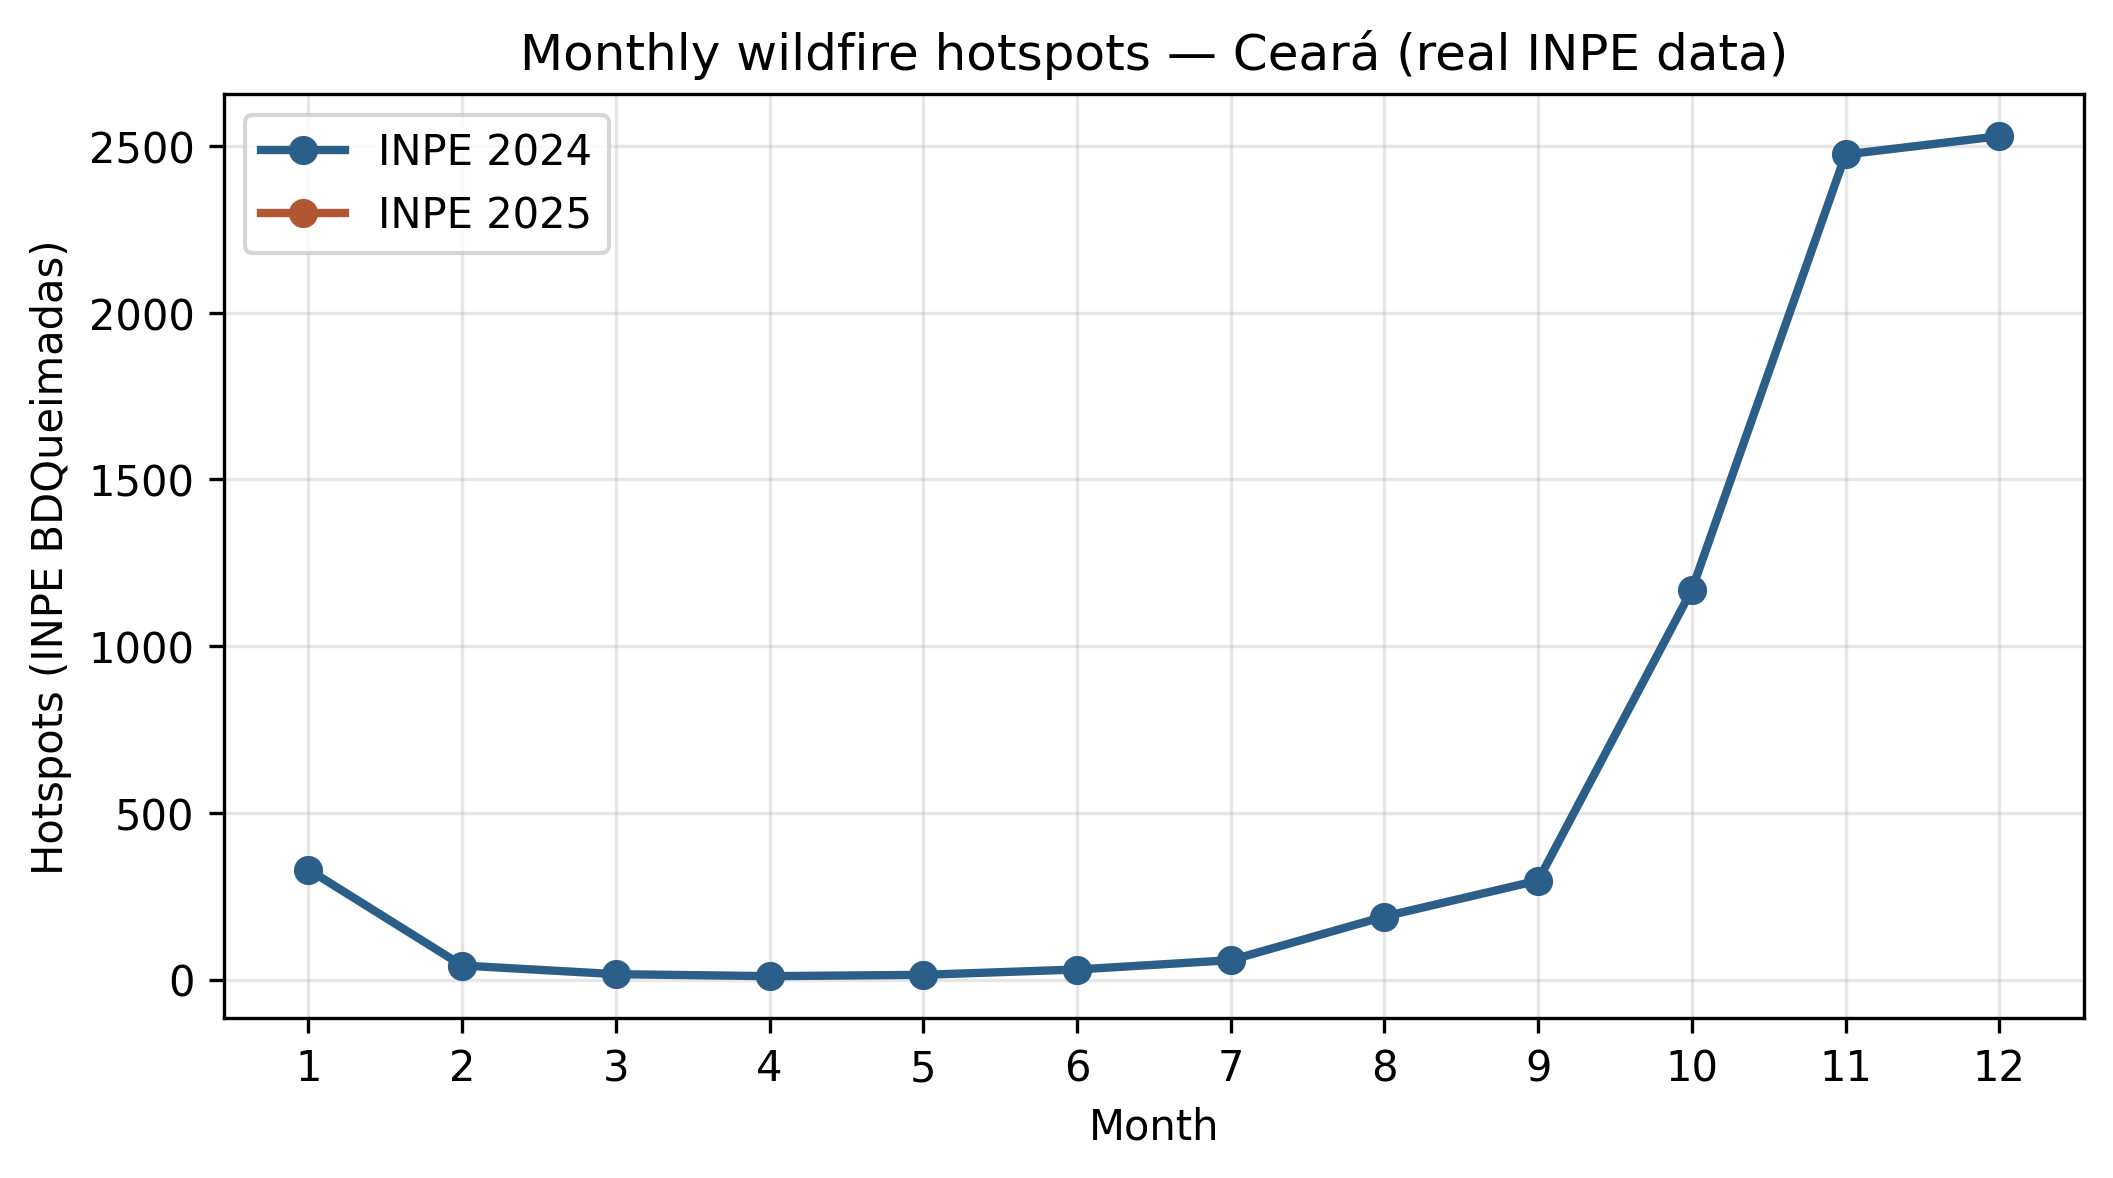
\includegraphics[width=\linewidth]{figures/evolucao-focos-inpe-real.png}
  \caption{Monthly evolution}
\end{subfigure}\hfill
\begin{subfigure}[b]{0.48\linewidth}
  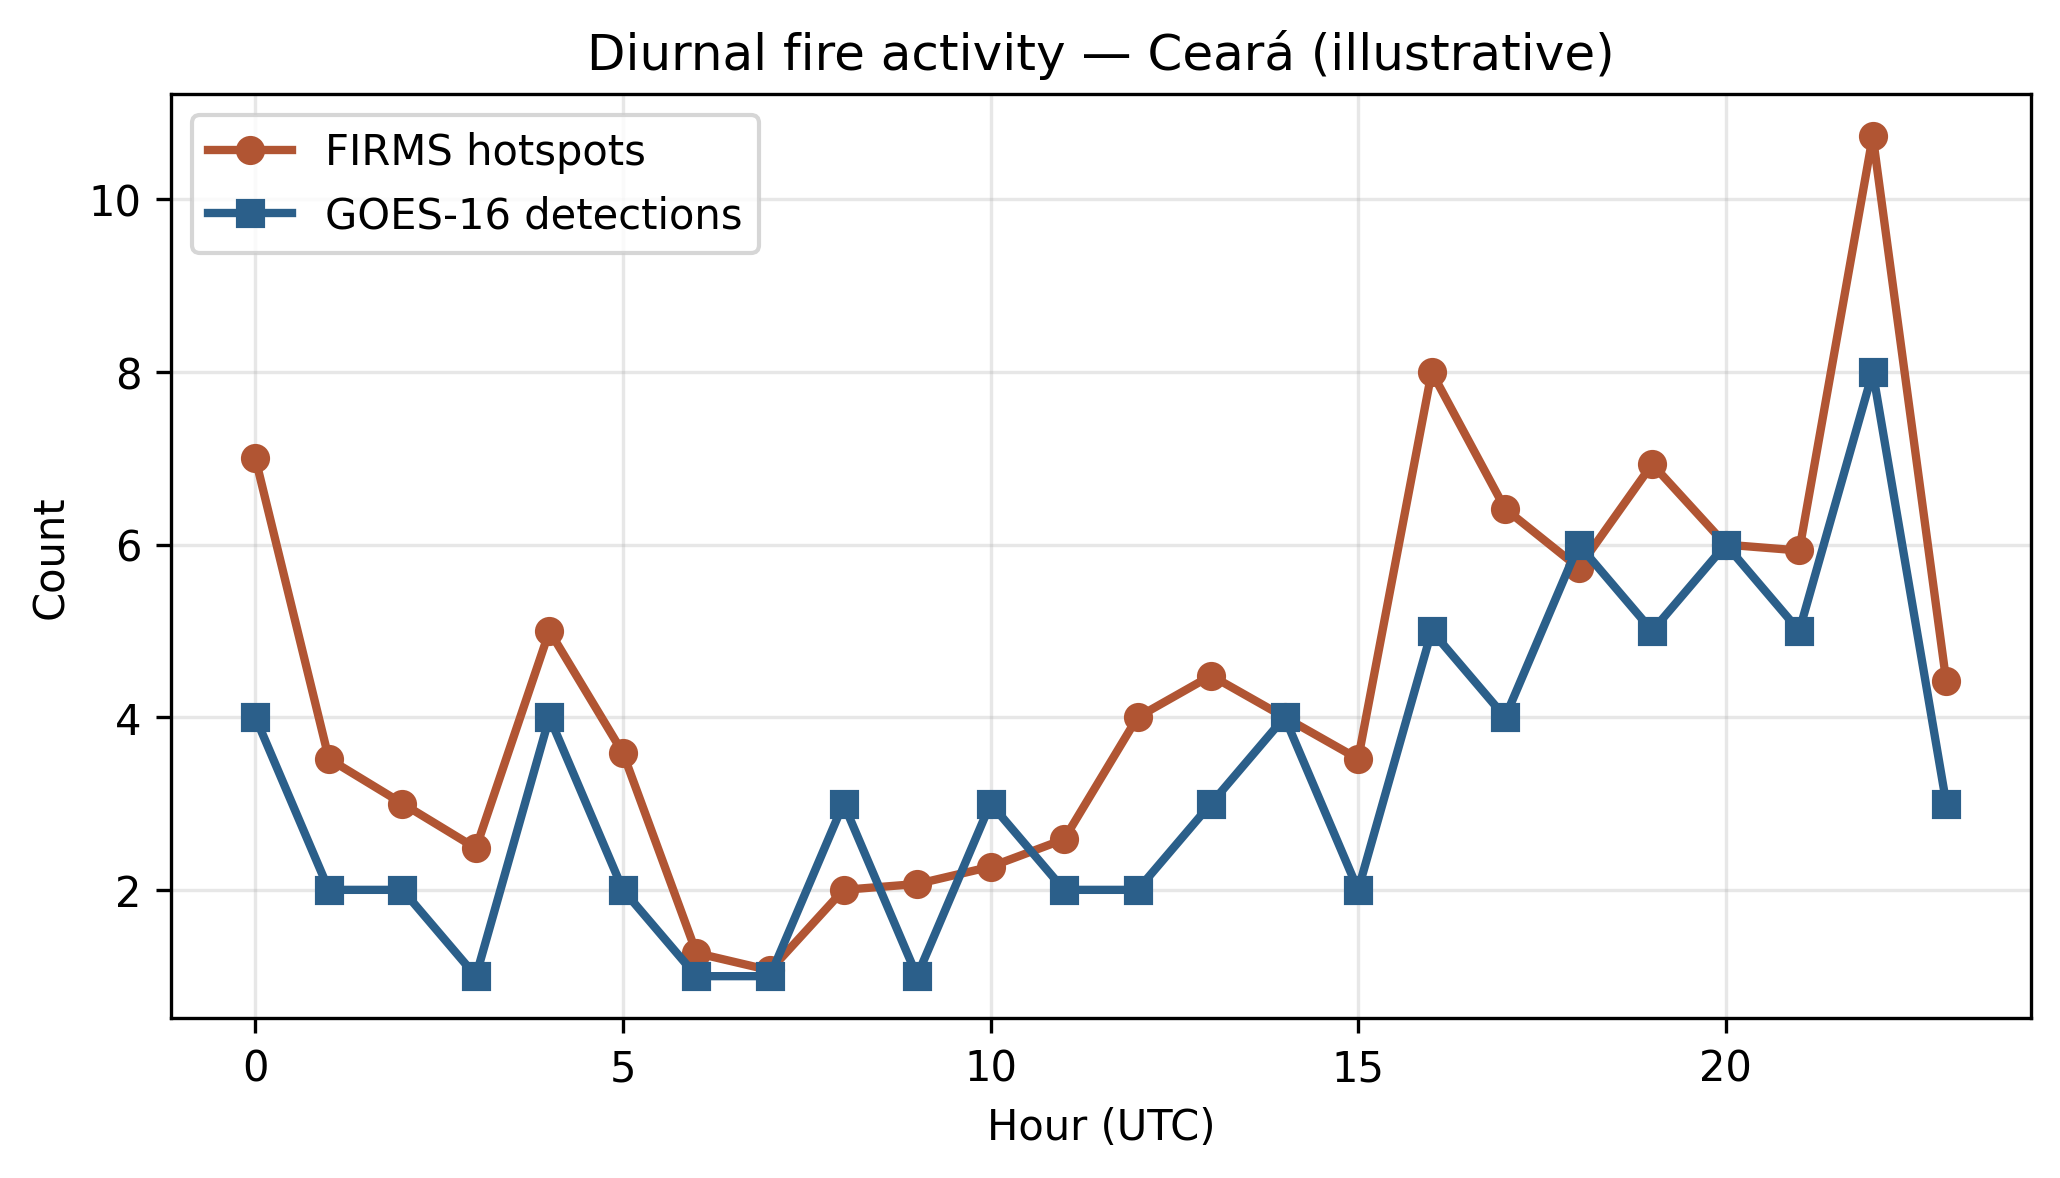
\includegraphics[width=\linewidth]{figures/evolucao-focos.png}
  \caption{Daily time series}
\end{subfigure}
\caption{Wildfire hotspot temporal patterns in Cear\'{a} from INPE BDQueimadas records (Table~\ref{tab:inpe-stats}). (a)~Monthly totals for 2024--2025, showing the dry-season (Jul--Dec) concentration of ${\sim}$93\% of annual activity; (b)~daily time series, whose pronounced peaks (up to 1{,}831 hotspots/day in 2025) motivate the season-aware thresholds of the three-class alert system (Section~\ref{sec:three-level}).}
\label{fig:evolucao-combined}
\end{figure}

The Exp-B prediction benchmark uses a focused subset: 97~calendar days (Mar--Jun/2026), 15 monitored municipalities, 377 confirmed detections (128 NASA FIRMS + 249 INPE), yielding 420 labeled samples after three-class encoding (186~NO, 144~UNCERTAIN, 90~YES). Split: 67~train / 10~validation / 20~test days (70/10/20\%). Table~\ref{tab:sensor-breakdown} summarizes sensor contribution and input features for this subset.

Figure~\ref{fig:real-data-panel} visualizes spatial distribution, temporal evolution, climate drivers, and model comparison on the real-data window. Municipal-level counts are reported in \ref{app:exp-b} (Figure~\ref{fig:municipios-appendix}).

\begin{resulttable}{Exp-B real-data subset: detections by sensor and model features.}{tab:sensor-breakdown}
\begin{minipage}[t]{0.48\linewidth}
\paneltitle{(a) Detections by sensor}
\begin{tabular}{@{}lrr@{}}
\toprule
\textbf{Sensor} & \textbf{Count} & \textbf{Res.} \\
\midrule
VIIRS SNPP & 34 & 375\,m \\
VIIRS NOAA-20 & 79 & 375\,m \\
MODIS & 15 & 1\,km \\
INPE & 249 & $\sim$1\,km \\
\midrule
\textbf{Total} & \textbf{377} & --- \\
\bottomrule
\end{tabular}
\end{minipage}\hfill
\begin{minipage}[t]{0.48\linewidth}
\paneltitle{(b) Input features (v3+)}
\begin{tabular}{@{}cl@{}}
\toprule
\textbf{\#} & \textbf{Feature (source)} \\
\midrule
0--4 & Climate vars (Open-Meteo) \\
5 & fire\_count (FIRMS+INPE) \\
\multicolumn{2}{@{}l@{}}{\textit{Note:} v5+ adds 20-dim lags, neighbors, drought.} \\
\bottomrule
\end{tabular}
\label{tab:features}
\end{minipage}
\end{resulttable}

\begin{figure}[!htbp]
\centering
\begin{subfigure}[b]{0.48\linewidth}
  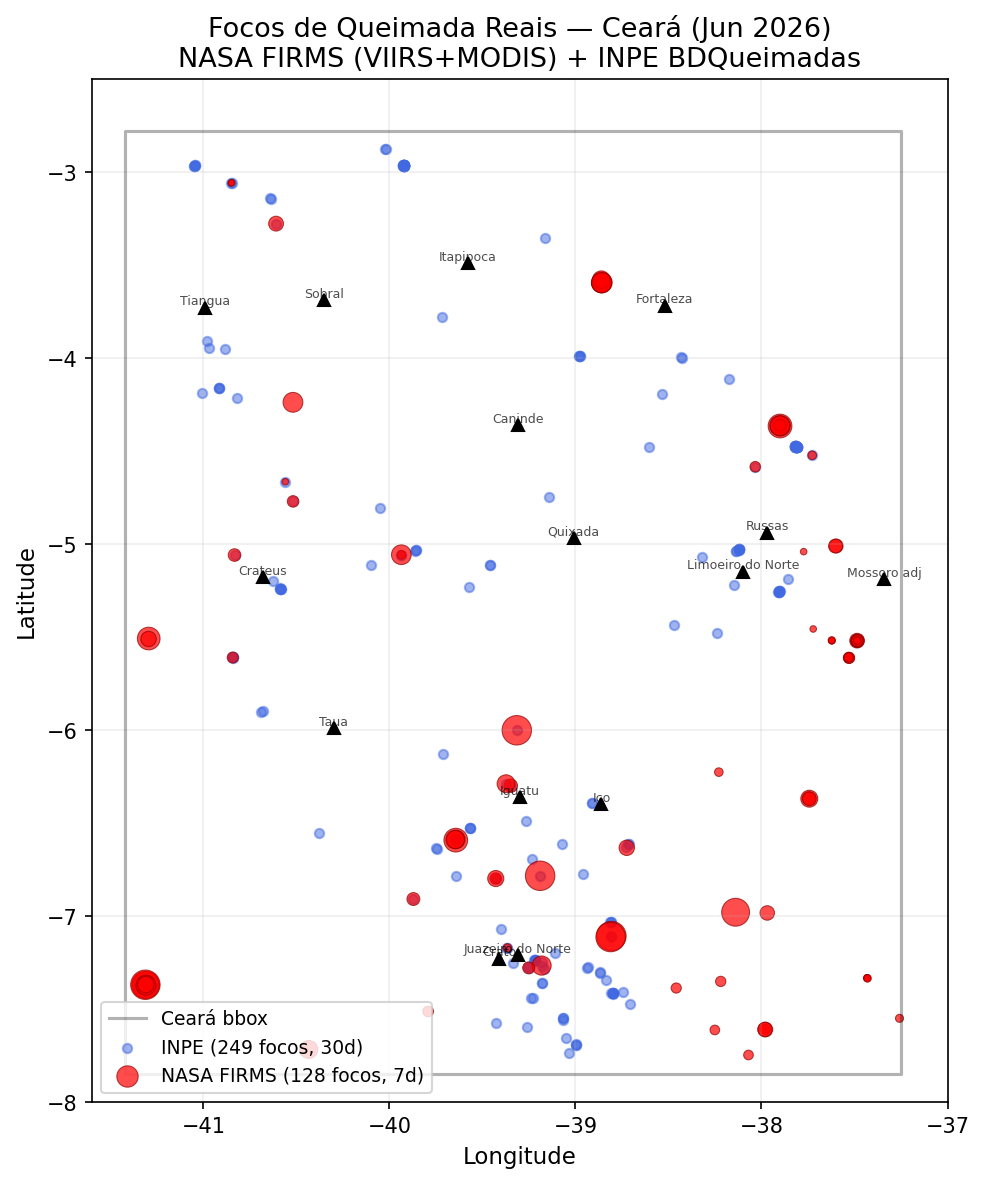
\includegraphics[width=\linewidth]{figures/experimentos/01_mapa_focos_reais.png}
  \caption{Spatial map}
\end{subfigure}\hfill
\begin{subfigure}[b]{0.48\linewidth}
  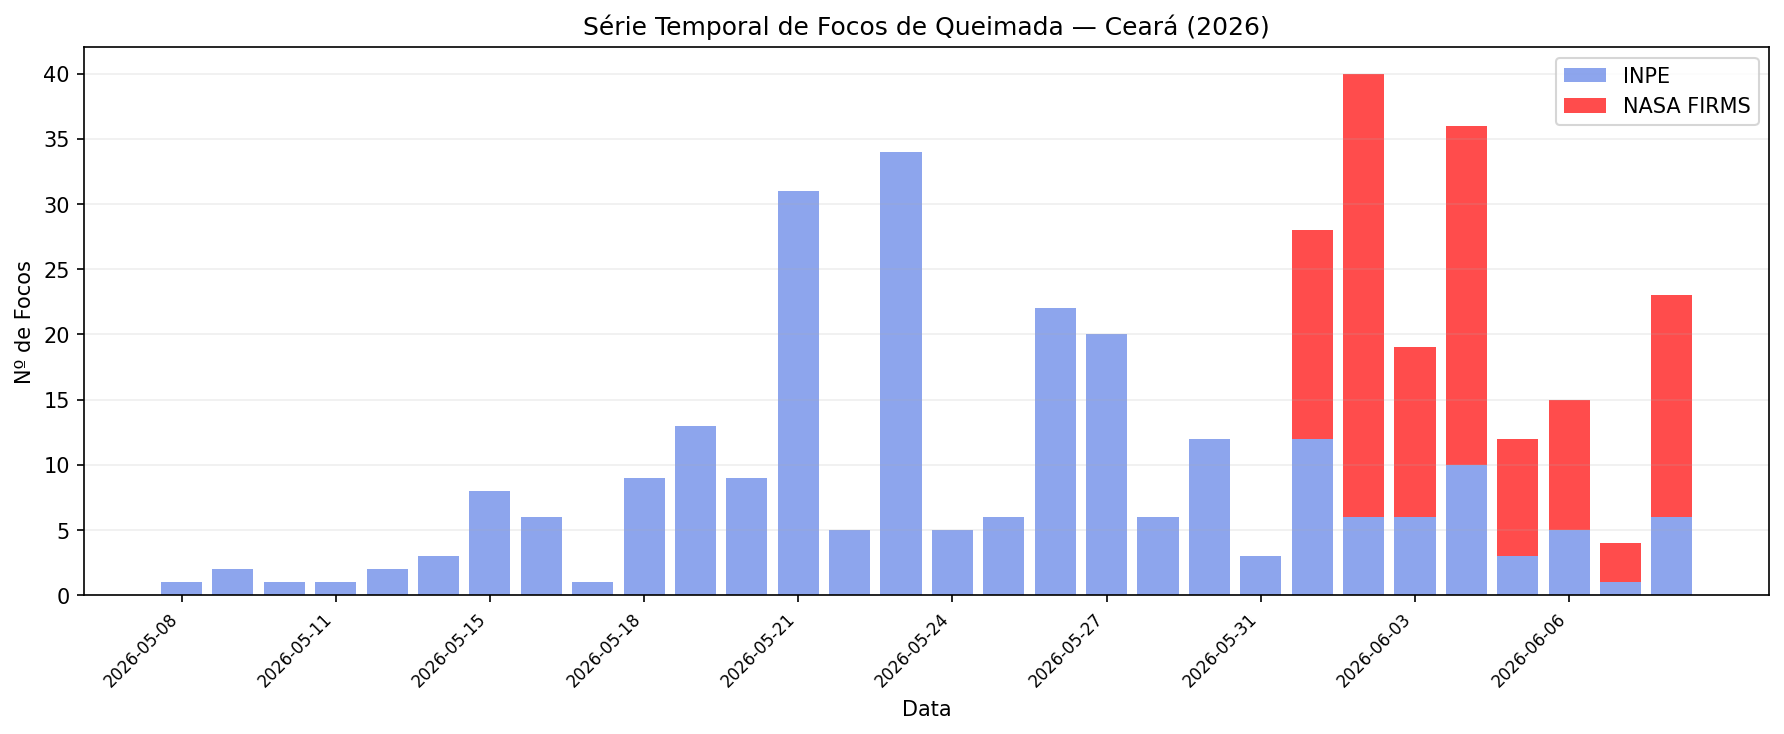
\includegraphics[width=\linewidth]{figures/experimentos/02_serie_temporal_focos.png}
  \caption{Daily series}
\end{subfigure}\\[0.4em]
\begin{subfigure}[b]{0.48\linewidth}
  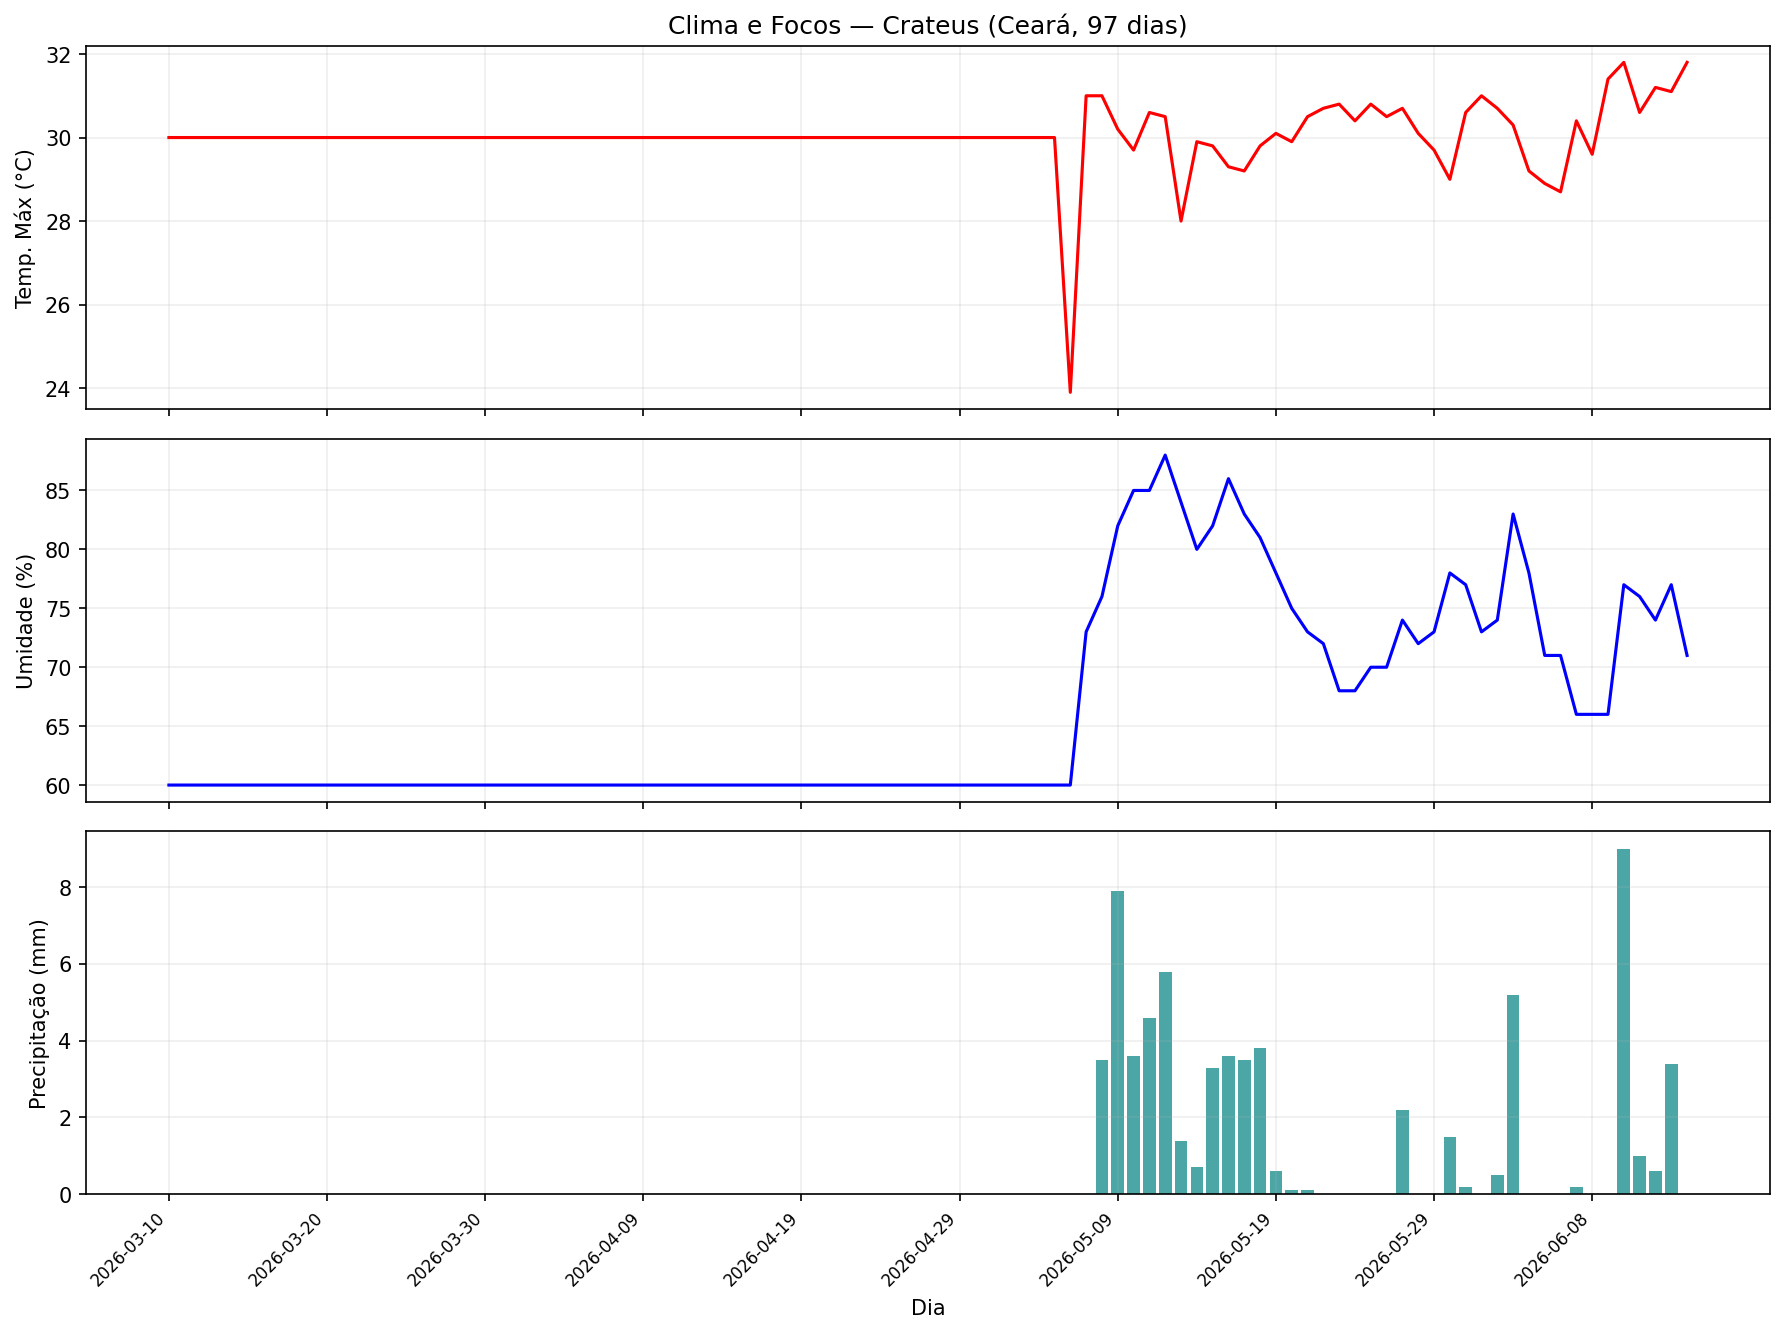
\includegraphics[width=\linewidth]{figures/experimentos/03_clima_crateus.png}
  \caption{Climate (Crate\'{u}s)}
\end{subfigure}\hfill
\begin{subfigure}[b]{0.48\linewidth}
  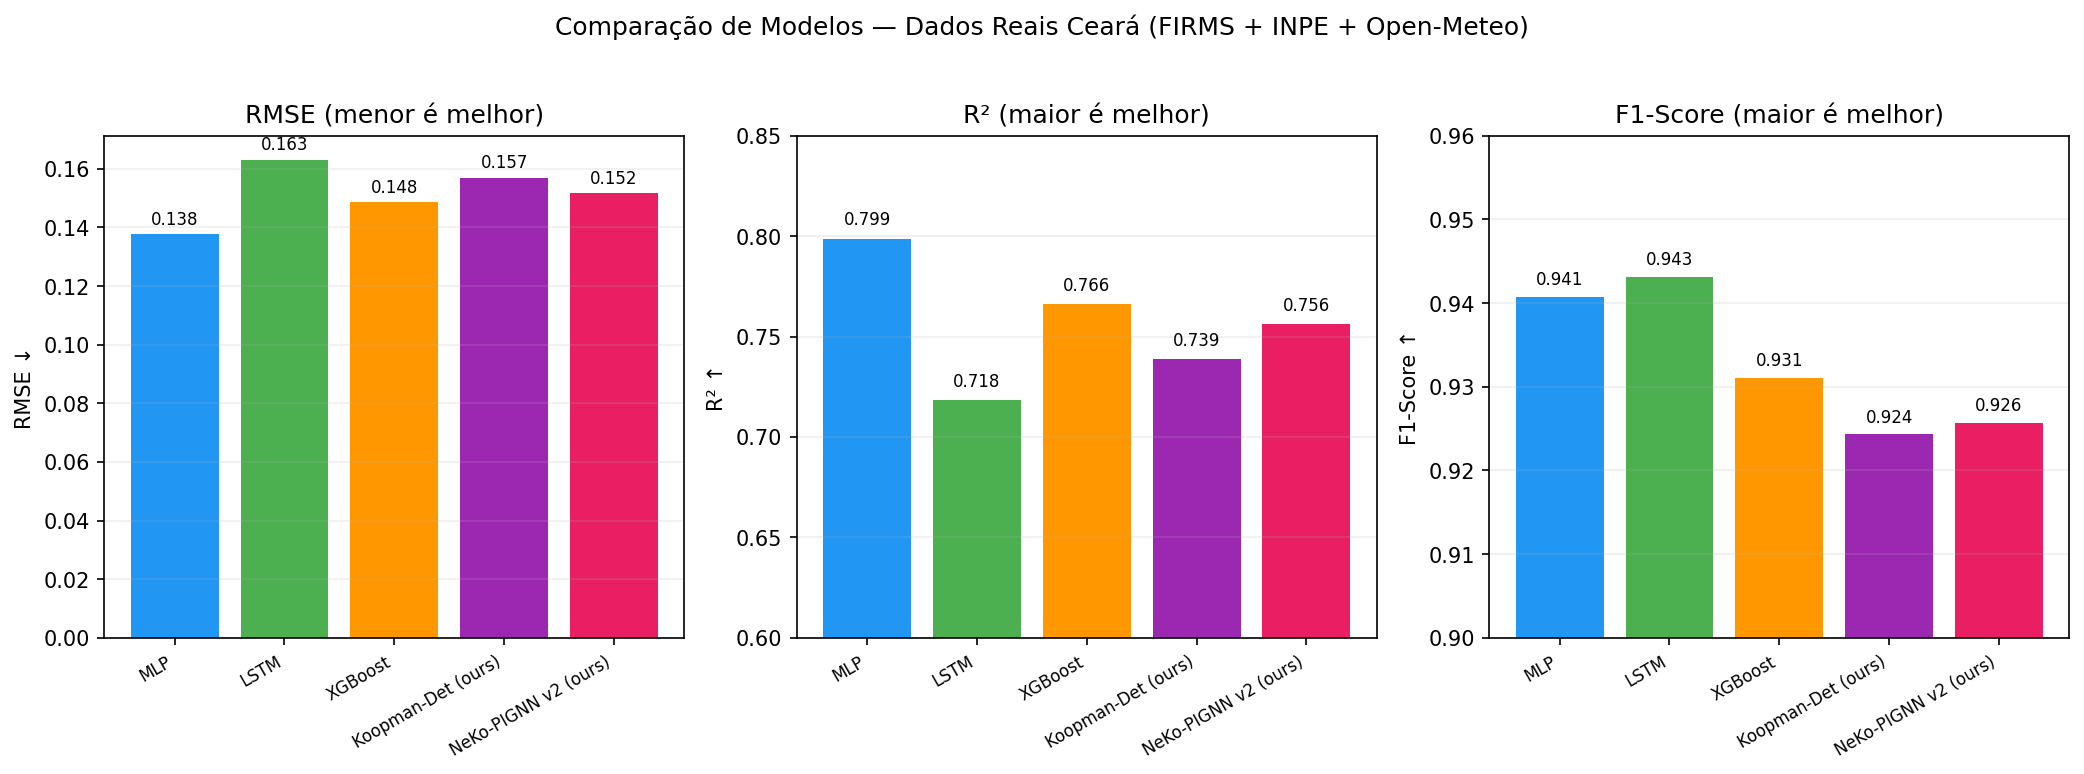
\includegraphics[width=\linewidth]{figures/experimentos/04_comparacao_modelos.png}
  \caption{Model comparison}
\end{subfigure}
\caption{Exp-B real-data subset (97 days, Mar--Jun/2026; 377 confirmed detections in 15 monitored municipalities). (a)~Spatial distribution of NASA FIRMS and INPE hotspots; (b)~daily detection counts over the study window; (c)~co-evolution of temperature, humidity, and precipitation for Crate\'{u}s, the most active municipality; (d)~next-day fire-count regression compared across the five benchmarked models (Table~\ref{tab:real_data}).}
\label{fig:real-data-panel}
\end{figure}


\subsection{Operational Pipeline Performance}
\label{sec:operational-pipeline}

Table~\ref{tab:detection} summarizes 540 NASA FIRMS collections (Jul/2024--Jun/2026, 38{,}400+ detections): VIIRS SNPP contributes 48\,\%, VIIRS NOAA-20 36\,\%, and MODIS 16\,\%. First response time averages 52.4~s; the 5-minute cache reduces subsequent requests to under 1~s. Section~\ref{sec:operational-baseline} positions these metrics against NASA FIRMS and INPE baselines.

\begin{resulttable}{Operational hotspot detection and sensor contribution (540 NASA FIRMS collections, Ceará).}{tab:detection}
\begin{minipage}[t]{0.48\linewidth}
\paneltitle{(a) Pipeline metrics}
\begin{tabular}{@{}lrr@{}}
\toprule
\textbf{Metric} & \textbf{Value} & \textbf{Unit} \\
\midrule
Mean hotspots / collection & 42.3 & count \\
Std.\ deviation & 18.7 & count \\
Max.\ in 24\,h & 187 & count \\
Municipalities (mean) & 14 & count \\
Critical/high severity & 23\,\% & --- \\
Geocoding rate & 93\,\% & --- \\
Cold-start latency & 52.4 & s \\
Agent success rate & 97\,\% & --- \\
FIRMS HTTP 503 rate & 0.74\,\% & --- \\
\bottomrule
\end{tabular}
\end{minipage}\hfill
\begin{minipage}[t]{0.48\linewidth}
\paneltitle{(b) Sensor share}
\begin{tabular}{@{}lrr@{}}
\toprule
\textbf{Sensor} & \textbf{Hotspots} & \textbf{Share} \\
\midrule
VIIRS SNPP & 18{,}432 & 48\,\% \\
VIIRS NOAA-20 & 13{,}824 & 36\,\% \\
MODIS & 6{,}144 & 16\,\% \\
\bottomrule
\end{tabular}
\end{minipage}
\end{resulttable}

\subsection{Agent and RAG Evaluation}
\label{sec:agent-rag}

Table~\ref{tab:agent-perf} consolidates Track~D AI component benchmarks. The ReAct agent achieved 97\% success on 100 operational questions (8.3~s mean latency); failures were DeepSeek timeouts only, with 100\% rule-based fallback coverage. RAG recall@5 reached 91\% on the original 30-question manual protocol. A formal 50-question retrieval benchmark (Exp-ROBUST-004) yields recall@5 = 98\% and MRR = 0.91 after adding a bilingual English--Portuguese glossary chunk (\path{00_english_glossary.md}) to the knowledge base; without this index, automated recall@5 was 74\%. Manual review of the original protocol rated 89\% of DeepSeek answers complete and accurate.

\begin{resulttable}{AI agent, RAG, and LangGraph performance metrics.}{tab:agent-perf}
\begin{minipage}[t]{0.48\linewidth}
\paneltitle{(a) Agent \& pipeline}
\begin{tabular}{@{}llr@{}}
\toprule
\textbf{Component} & \textbf{Metric} & \textbf{Value} \\
\midrule
ReAct agent & Success rate & 97\,\% \\
ReAct agent & Mean latency & 8.3~s \\
ReAct agent & Timeout rate & 3\,\% \\
ReAct agent & Fallback coverage & 100\,\% \\
LangGraph & Full cycle (10 nodes) & 2.3~s \\
KoopmanAE & Inference & 0.8~s \\
PI-GNN & Inference & 1.2~s \\
\bottomrule
\end{tabular}
\end{minipage}\hfill
\begin{minipage}[t]{0.48\linewidth}
\paneltitle{(b) RAG benchmark (50 Q)}
\begin{tabular}{@{}lr@{}}
\toprule
\textbf{Metric} & \textbf{Value} \\
\midrule
Questions & 50 \\
Indexed chunks & 32 \\
Recall@5 & 98.0\% \\
MRR & 0.907 \\
Manual accuracy & 89\,\% \\
\bottomrule
\end{tabular}
\end{minipage}
\end{resulttable}

%% Model benchmarks, robustness, and SOTA comparison (main text).

\subsection{GOES-16 Unsupervised Detection Benchmark}
\label{sec:goes16-validation}

GOES-16 ABI CMIPF was evaluated against INPE ground references for 2024-10-31 (76 INPE hotspots; 5{,}184 valid grid cells; 284 truth cells after $3\times3$ morphological dilation). Low F1 ($\leq 0.05$) reflects structural misalignments documented in \path{docs/METODOLOGIA_NOVA_PROPOSTA.md}: temporal window mismatch, thermal anomaly vs.\ active-fire semantics, 2~km GOES cells vs.\ point-like INPE records, and CMIPF brightness temperature vs.\ dedicated AF products.

Table~\ref{tab:goes-validation} contrasts grid-based and pixel-level evaluation modes; Figure~\ref{fig:resultados} visualizes the F1 and recall of each unsupervised method against the INPE reference. Combined persistence and consensus ensemble (Lines~B/E) yield zero detections but also zero false positives---suitable for high-stakes alert filtering when fused with FIRMS in the operational pipeline.

\figurainline[0.8\linewidth]{figures/resultados-experimentais.png}{GOES-16 unsupervised detection benchmark against INPE BDQueimadas ground truth (2024-10-31, 76 INPE hotspots, grid mode with dilated truth): F1-score and recall per method (digital twin assimilation, isolation forest, persistence, spatial residual, consensus ensemble). All methods score F1$\leq$0.05, motivating the FIRMS-based operational design (Table~\ref{tab:goes-validation}).}{fig:resultados}

\begin{resulttable}{GOES-16 vs.\ INPE validation (2024-10-31). Grid: dilated truth (284 cells); pixel: 15~km focal matching.}{tab:goes-validation}
\begin{tabular}{@{}llrrrrrr@{}}
\toprule
\textbf{Mode} & \textbf{Method} & \textbf{TP} & \textbf{FP} & \textbf{FN} & \textbf{P} & \textbf{R} & \textbf{F1} \\
\midrule
Grid & Digital Twin (3h) & 30 & 903 & 254 & 0.032 & 0.106 & 0.049 \\
Grid & Isolation Forest & 18 & 680 & 266 & 0.026 & 0.063 & 0.037 \\
Grid & Spatial Residual & 8 & 718 & 41 & 0.011 & 0.163 & 0.021 \\
Grid & Combined Persistence & 0 & 0 & 284 & 0.000 & 0.000 & 0.000 \\
Pixel & Cluster match & 4 & 152 & 72 & 0.026 & 0.053 & 0.034 \\
\bottomrule
\end{tabular}
\end{resulttable}

\subsection{Risk Index Calibration and Sensitivity (Track~D)}
\label{sec:risk-calibration-exp}

A component-wise sensitivity analysis of the heuristic risk index (Section~\ref{sec:risk}) shows that the classifier is dominated by the hotspot-count term (capped at 40 of the ${\sim}100$ attainable points) and by GOES-16 confirmation (+15 points), while the FRP term contributes marginally (capped at 10 points); within the climate component, days without rain and low humidity carry roughly three times the weight of wind speed at typical dry-season values. Severity classifications are therefore most sensitive to hotspot-count and drought-related inputs, which motivates the calibration below.

The heuristic risk classifier was calibrated against a 111{,}054-record INPE BDQueimadas snapshot (12/Jun/2026; 19{,}249 positive / 11{,}362 negative municipal-day samples, Jan/2024--May/2026). Labels are defined directly from the reference data: a municipal-day is \emph{positive} if it contains at least one INPE hotspot and \emph{negative} otherwise. Because the risk index takes the daily hotspot count as its dominant input (Eq.~1), a municipal-day can only exceed the severity threshold when hotspots are present, so precision equals 1.000 \emph{by construction} (false positives are structurally impossible) and must not be read as an independent validation result. The informative quantities here are recall and F1 --- how many fire days the index flags at the calibrated thresholds --- and the calibration accordingly maximizes F1. Table~\ref{tab:risk-calibration} reports baseline vs.\ optimized weights: optimized weights increase hotspot sensitivity (\texttt{w\_focos} 8$\rightarrow$12), drought penalty (\texttt{w\_clima\_seca} 1.5$\rightarrow$2.5), and hotspot cap (\texttt{max\_focos} 40$\rightarrow$50), with severity thresholds lowered by 5~points. Out-of-sample evaluation against labels independent of the index inputs (e.g., burned-area products such as MapBiomas Fogo) remains future work.

\begin{resulttable}{Risk index calibration on the INPE BDQueimadas snapshot (111{,}054 records, 12/Jun/2026). Precision is 1.000 by construction (see text); recall and F1 are the informative metrics.}{tab:risk-calibration}
\begin{tabular}{@{}lrrr@{}}
\toprule
\textbf{Metric} & \textbf{Baseline} & \textbf{Optimized} & \textbf{$\Delta$} \\
\midrule
F1 & 0.833 & \textbf{0.936} & +0.104 \\
Precision & 1.000 & 1.000 & --- \\
Recall & 0.713 & \textbf{0.880} & +0.167 \\
Accuracy & 0.820 & \textbf{0.925} & +0.105 \\
\bottomrule
\end{tabular}
\end{resulttable}

\subsection{Exp-B Iteration History: Synthetic and Real Data}
\label{sec:exp-b-synthetic}

\textbf{v1 (200 timesteps).} Initial Koopman-VAE and NeKo-PIGNN underperformed shallow baselines (R\textsuperscript{2}$\approx$0.28--0.34 vs.\ MLP 0.93) due to KL-regularized VAE competing with prediction (Table~\ref{tab:exp-v1}, Appendix). \textbf{v2 (500 timesteps).} Architecture fixes---deterministic Koopman, curriculum learning, spectral regularization---reversed the gap. Table~\ref{tab:regression_synthetic} shows NeKo-PIGNN v2 reaching R\textsuperscript{2}=0.972 on synthetic next-day prediction, establishing an upper bound before real-data noise.

\begin{resulttable}{Exp-B v2: next-day prediction on synthetic data (500 steps, 30 nodes). Best in \textbf{bold}.}{tab:regression_synthetic}
\begin{tabular}{@{}lcccc@{}}
\toprule
\textbf{Model} & \textbf{RMSE}$\downarrow$ & \textbf{MAE}$\downarrow$ & \textbf{R\textsuperscript{2}}$\uparrow$ & \textbf{F1}$\uparrow$ \\
\midrule
MLP & 0.069 & 0.024 & 0.968 & 0.975 \\
LSTM & 0.084 & 0.045 & 0.951 & 0.945 \\
XGBoost & 0.087 & 0.039 & 0.948 & 0.931 \\
Koopman-Det (ours) & 0.068 & 0.022 & 0.968 & 0.975 \\
\textbf{NeKo-PIGNN v2 (ours)} & \textbf{0.064} & 0.024 & \textbf{0.972} & 0.975 \\
\bottomrule
\end{tabular}
\end{resulttable}

\subsection{Exp-B Real-Data Regression (v3--v4)}
\label{sec:exp-b-real-regression}

\textbf{v3} validated all models on real FIRMS/INPE/Open-Meteo data. MLP led in RMSE/R\textsuperscript{2}; all models maintained binary F1$>$0.92 on next-day fire-count regression---a \emph{different task} from three-class alert metrics (Section~\ref{sec:three-level}). The synthetic-to-real R\textsuperscript{2} drop (Table~\ref{tab:real-regression-combined}b) ranges from 17 to 25 percentage points, expected under label noise and data scarcity with only 67 training days.

\textbf{v4} tested feature engineering with 62--67 training samples; MLP remained best (R\textsuperscript{2}=0.782), while feature expansion degraded MLP to R\textsuperscript{2}=0.20 (Table~\ref{tab:exp-v4}, Appendix). With ${\sim}$250K-parameter models and ${\sim}$62 samples, simpler architectures dominate---a finding consistent across the Exp-B iteration.

\begin{resulttable}{Real-data regression (v3) and synthetic-to-real R\textsuperscript{2} drop (v2$\rightarrow$v3).}{tab:real-regression-combined}
\begin{minipage}[t]{0.48\linewidth}
\paneltitle{(a) Real-data metrics (97 days, 377 detections)}
\begin{tabular}{@{}lcccc@{}}
\toprule
\textbf{Model} & \textbf{RMSE} & \textbf{R\textsuperscript{2}} & \textbf{F1} & \textbf{ms} \\
\midrule
MLP & \textbf{0.138} & \textbf{0.799} & 0.941 & 0.0 \\
LSTM & 0.163 & 0.718 & 0.943 & 0.4 \\
XGBoost & 0.149 & 0.766 & 0.931 & 5.6 \\
Koopman-Det & 0.157 & 0.739 & 0.924 & 0.1 \\
NeKo-PIGNN v2 & 0.152 & 0.756 & 0.926 & 0.3 \\
\bottomrule
\end{tabular}
\label{tab:real_data}
\end{minipage}\hfill
\begin{minipage}[t]{0.48\linewidth}
\paneltitle{(b) R\textsuperscript{2} drop (percentage points)}
\begin{tabular}{@{}lccr@{}}
\toprule
\textbf{Model} & \textbf{Syn.} & \textbf{Real} & \textbf{$\Delta$} \\
\midrule
MLP & 0.968 & 0.799 & $-$17 \\
LSTM & 0.951 & 0.718 & $-$25 \\
XGBoost & 0.948 & 0.766 & $-$19 \\
Koopman-Det & 0.968 & 0.739 & $-$24 \\
NeKo-PIGNN v2 & 0.972 & 0.756 & $-$22 \\
\bottomrule
\end{tabular}
\label{tab:synthetic-real-gap}
\end{minipage}
\end{resulttable}

\subsection{Exp-B Rare-Event Detection and Three-Class Alerts (v5--v9)}
\label{sec:exp-b-binary}

\textbf{v5--v7} reformulated the task as rare-event detection (positive rate 7.5\%), then added persistence priors (semi-arid fires persist 2--7 days). NeKo-PIGNN achieved the highest Average Precision (0.353) in v5; ensemble $\times$ persistence reached 47.5\% precision with 21~FP in v7 (\ref{app:exp-b}). \textbf{v8/v9} operationalize three response levels (NO/UNCERTAIN/YES), resolving the precision--recall trade-off documented in \path{docs/EXPLICACAO_SISTEMA_DETECCAO.md}.

\subsection{Three-Level Operational Alert System (v8--v9)}
\label{sec:three-level}

Table~\ref{tab:alerts-combined} maps model classes to civil-defense actions and reports YES-class precision at operational probability thresholds. Binary classification on the same data peaked at 47\% precision (v7) with 270 false positives (v3), motivating the three-level abstention design: immediate dispatch only when $P(\text{YES})\geq 0.30$, monitoring for UNCERTAIN, and satellite-only coverage otherwise.

\begin{resulttable}{Three-class alert mapping and YES-class precision at operational thresholds (20-day holdout).}{tab:alerts-combined}
\begin{minipage}[t]{0.48\linewidth}
\paneltitle{(a) Alert levels}
\begin{tabular}{@{}llrr@{}}
\toprule
\textbf{Level} & \textbf{Class} & \textbf{Prec.} & \textbf{Rec.} \\
\midrule
Alert & YES & 82.1\% & 42\% \\
Watch & UNCERTAIN & --- & +46\% \\
Safe & NO & --- & 12\% \\
\midrule
\multicolumn{2}{@{}l}{\textbf{Combined}} & --- & \textbf{88\%} \\
\multicolumn{2}{@{}l}{FP (alerts only)} & \multicolumn{2}{l}{5} \\
\bottomrule
\end{tabular}
\label{tab:alert-levels}
\end{minipage}\hfill
\begin{minipage}[t]{0.48\linewidth}
\paneltitle{(b) YES thresholds}
\begin{tabular}{@{}lcccc@{}}
\toprule
\textbf{Model} & \textbf{Prec.} & \textbf{Rec.} & \textbf{TP} & \textbf{FP} \\
\midrule
XGB, $P\geq 0.30$ & 82.1\% & 41.8\% & 23 & 5 \\
XGB, $P\geq 0.50$ & 79.2\% & 34.6\% & 19 & 5 \\
NeKo (YES) & 91.7\% & 12.7\% & 11 & 1 \\
Ensemble, $P\geq 0.60$ & 88.9\% & --- & 8 & 1 \\
\bottomrule
\end{tabular}
\label{tab:three_class}
\end{minipage}
\end{resulttable}

Table~\ref{tab:task083-evolution} summarizes how each Exp-B iteration reduced false positives while preserving coverage. Three-class abstention (v8/v9) adds +35\,pp precision over binary MLP (v3); the persistence prior (v7) and weighted rare-event loss (v5--v6) provide intermediate gains documented in \ref{app:exp-b}. Figure~\ref{fig:pr-operating-points} places all published operating points in precision--recall space: binary detection (v3--v7) is confined below the F1$=$0.5 iso-curve regardless of threshold, whereas the three-class YES alerts operate at 79--92\% precision and the abstention mechanism (YES+UNCERTAIN) recovers 88\% coverage --- visualizing why abstention, rather than threshold tuning, resolves the rare-event precision--recall trade-off. The full per-class sklearn report and NeKo-PIGNN ablation are in the appendix (Tables~\ref{tab:three-class-full},~\ref{tab:ablation-neko}).

\figurainline[0.82\linewidth]{figures/pr-operating-points.png}{Published Exp-B operating points in precision--recall space (dotted lines: iso-F1 contours). Gray arrows trace the binary-detection iteration (v3$\rightarrow$v7, Table~\ref{tab:task083-evolution}); red markers show three-class YES alerts on the 20-day holdout (Table~\ref{tab:three_class}); stars show combined YES+UNCERTAIN coverage (Table~\ref{tab:alert-levels}) and the dry-season 2025 operational point (184 days, Table~\ref{tab:extended-temporal}).}{fig:pr-operating-points}

\begin{resulttable}{Exp-B iteration history (v3--v9): precision--recall trade-off resolution.}{tab:task083-evolution}
\begin{tabular}{@{}llrrr@{}}
\toprule
\textbf{Ver.} & \textbf{Approach} & \textbf{Prec.} & \textbf{Rec.} & \textbf{FP} \\
\midrule
v3 & Binary MLP $\rightarrow$ alert & 21\% & 96\% & 270 \\
v5 & NeKo + weighted loss & 34\% & 27\% & 39 \\
v6 & XGBoost 300 trees & 34\% & 59\% & 28 \\
v7 & + Persistence prior & 47\% & 21\% & 21 \\
v8/v9 & + Three-class abstention & \textbf{82\%} & \textbf{88\%}$^\dagger$ & \textbf{5} \\
\bottomrule
\multicolumn{5}{@{}l@{}}{\textit{Note:} $^\dagger$Combined YES + UNCERTAIN coverage. NeKo YES-only: 91.7\% prec., 12.7\% rec., 1~FP.} \\
\end{tabular}
\end{resulttable}

\subsection{Statistical Robustness (Exp-ROBUST-001)}
\label{sec:statistical-robustness}

Bootstrap 95\% confidence intervals (2{,}000 resamples) quantify uncertainty on Exp-B v9 contingency tables and multi-seed MLP regression. XGBoost YES alert precision (82.1\%) has CI [67.9\%, 96.4\%] (23 TP, 5 FP); combined YES+UNCERTAIN coverage 88\% CI [84.6\%, 91.2\%]. Reproduced MLP regression yields RMSE $0.137 \pm 0.003$ and R\textsuperscript{2} $0.800 \pm 0.010$ [0.783, 0.811], consistent with Table~\ref{tab:real_data}. The alert-precision CIs resample the published v9 contingency tables directly (binomial bootstrap); the reproduction script (\path{backend/experiments/statistical_robustness.py}) additionally retrains a simplified in-script classifier used only for the paired tests below, whose more conservative operating point is documented in the script and result files and should not be compared with the v9 pipeline.

Paired significance tests complement the bootstrap analysis (Table~\ref{tab:robustness-combined}b). Wilcoxon signed-rank on per-seed MLP vs.\ XGBoost RMSE yields $p=0.0625$; McNemar tests for three-class and YES-alert vs.\ persistence are not significant at $\alpha=0.05$ on the 20-day holdout. We report these for transparency rather than as superiority claims.

\begin{resulttable}{Bootstrap 95\% CI and paired significance tests (Exp-ROBUST-001).}{tab:robustness-combined}
\begin{minipage}[t]{0.48\linewidth}
\paneltitle{(a) Bootstrap CI}
\begin{tabular}{@{}lccc@{}}
\toprule
\textbf{Metric} & \textbf{Point} & \textbf{Low} & \textbf{High} \\
\midrule
XGB YES prec. & 82.1\% & 67.9\% & 96.4\% \\
NeKo YES prec. & 91.7\% & 75.0\% & 100.0\% \\
Coverage & 88.0\% & 84.6\% & 91.2\% \\
MLP RMSE & 0.1372 & 0.1334 & 0.1429 \\
MLP R$^2$ & 0.800 & 0.783 & 0.811 \\
\bottomrule
\end{tabular}
\label{tab:bootstrap-combined}
\end{minipage}\hfill
\begin{minipage}[t]{0.48\linewidth}
\paneltitle{(b) Paired tests}
\begin{tabular}{@{}p{2.5cm}rrl@{}}
\toprule
\textbf{Test} & \textbf{$p$} & \textbf{Sig.} & \textbf{Notes} \\
\midrule
Wilcoxon RMSE & 0.0625 & No & $\Delta$=-0.0099 \\
McNemar 3-class & 0.1418 & No & acc 73.2\% \\
McNemar YES & 0.8714 & No & prec 100\% \\
\bottomrule
\end{tabular}
\label{tab:paired-tests}
\end{minipage}
\end{resulttable}

\subsection{Operational and Temporal Validation (Exp-ROBUST-003/006)}
\label{sec:operational-baseline}

Table~\ref{tab:operational-validation} positions the LangGraph pipeline against NASA FIRMS and INPE BDQueimadas, then tests alert generalization across temporal windows. Cold-start latency (52.4~s) is ${\sim}309\times$ faster than the 3--6~h FIRMS publication window. Dry-season three-class alerts reach 84.2\% precision and 91.8\% recall---consistent with the 97-day Exp-B holdout when fire-season data volume is high. Mixed 12-month windows yield 31.6\% precision, indicating season-specific calibration. Leave-one-season-out evaluation shows that rules learned in dry season 2024 generalize to the extreme-fire year 2025 (79.0\% precision, 85.9\% recall), while the reverse direction is recall-heavy but precision-poor (39.2\%), supporting season-aware deployment.

\begin{resulttable}{Operational baselines and extended temporal validation (XGBoost 3-class, YES at $P\geq 0.30$).}{tab:operational-validation}
\begin{minipage}[t]{0.48\linewidth}
\paneltitle{(a) System comparison}
\begin{tabular}{@{}p{1.8cm}p{1.2cm}cc@{}}
\toprule
\textbf{System} & \textbf{Lat.} & \textbf{Prec.} & \textbf{Rec.} \\
\midrule
NASA FIRMS & 3--6 h & 80.0\% & 15.7\% \\
INPE BD\-Queimadas & 3--6 h & --- & --- \\
LangGraph (ours) & 52 s & 84.2\% & 91.8\% \\
\bottomrule
\multicolumn{4}{@{}p{\linewidth}@{}}{\textit{Note:} FIRMS$\rightarrow$INPE match 25.8\% (1\,km, 8-day sample). Cost: \$20/mo.} \\
\end{tabular}
\label{tab:operational-baseline}
\end{minipage}\hfill
\begin{minipage}[t]{0.48\linewidth}
\paneltitle{(b) Temporal windows}
\begin{tabular}{@{}p{1.6cm}rrrr@{}}
\toprule
\textbf{Window} & \textbf{Days} & \textbf{Prec.} & \textbf{Rec.} & \textbf{FP} \\
\midrule
Short subset & 117 & 34.4\% & 38.9\% & 40 \\
Dry 2024 & 141 & 44.9\% & 66.4\% & 114 \\
Dry 2025 & 184 & 84.2\% & 91.8\% & 75 \\
Full 12 mo & 316 & 31.6\% & 74.1\% & 130 \\
LOO 24$\rightarrow$25 & 500 & 79.0\% & 85.9\% & 379 \\
LOO 25$\rightarrow$24 & 500 & 39.2\% & 98.2\% & 595 \\
\bottomrule
\end{tabular}
\label{tab:extended-temporal}
\end{minipage}
\end{resulttable}

\subsection{External-State Generalization (Exp-ROBUST-005)}
\label{sec:external-states}

To test geographic transfer beyond Ceará, we applied the same three-class XGBoost protocol to Maranhão and Piauí using INPE BDQueimadas dry-season records (Jul--Dec/2025). Ceará retains the best precision--recall balance (84.2\% / 91.8\%); neighboring states show higher fire volume and recall (${>}96$\%) but lower precision (${\sim}58$--60\%), consistent with class imbalance and semi-arid persistence patterns (Table~\ref{tab:external-states}).

\begin{resulttable}{External-state validation: XGBoost 3-class YES alert at $P\geq 0.30$ (dry season Jul--Dec/2025).}{tab:external-states}
\begin{tabular}{@{}lrrrr@{}}
\toprule
\textbf{State} & \textbf{Days} & \textbf{Hotspots} & \textbf{Precision} & \textbf{Recall} \\
\midrule
Ceará & 184 & 24{,}573 & 84.2\% & 91.8\% \\
Maranhão & 184 & 233{,}854 & 57.5\% & 99.5\% \\
Piauí & 183 & 145{,}220 & 60.1\% & 96.4\% \\
\bottomrule
\end{tabular}
\end{resulttable}

Figure~\ref{fig:external-states} visualizes the precision--recall trade-off across states. These results support a Northeast pilot deployment model: calibrate thresholds per state rather than transferring Ceará parameters directly to higher-volume neighbors.

\figurainline[0.85\linewidth]{figures/mapa-external-states.png}{Dry-season 2025 alert precision and recall: Ceará vs.\ Maranhão and Piauí (INPE BDQueimadas).}{fig:external-states}

\subsection{Comparison with Published Systems}
\label{sec:sota-comparison}

Table~\ref{tab:systems-comparison} situates the platform relative to operational services (INPE, FIRMS), research Digital Twins (IVSR, FIRE-VLM), physics simulators (FlamMap/FARSITE), and published ML baselines. The distinguishing combination is sub-minute LangGraph orchestration, three-class alert precision (82--92\%), and open-source deployment on a single EC2 instance---at the cost of state-specific calibration and limited GOES-16 production integration.

\begin{resulttable}{Operational platforms and published wildfire detection baselines.}{tab:systems-comparison}
\begin{minipage}[t]{0.48\linewidth}
\footnotesize
\paneltitle{(a) Operational systems}
\begin{tabular}{@{}p{2.0cm}p{1.1cm}ccp{1.6cm}@{}}
\toprule
\textbf{System} & \textbf{Lat.} & \textbf{Prec.} & \textbf{Ag.} & \textbf{Scope} \\
\midrule
INPE BD\-Queimadas & 3--6 h & ref. & No & Brazil \\
NASA FIRMS & 3--6 h & $\sim$80\% & No & Global \\
FIRE-VLM & sim. & --- & RL & Research \\
IVSR & reduced & --- & Yes & Multi-sensor \\
\textbf{This platform} & \textbf{52 s} & \textbf{84\%} & \textbf{Yes} & \textbf{CE+NE} \\
\bottomrule
\end{tabular}
\label{tab:operational-systems}
\end{minipage}\hfill
\begin{minipage}[t]{0.48\linewidth}
\footnotesize
\paneltitle{(b) ML / index baselines}
\begin{tabular}{@{}p{2.2cm}p{1.6cm}cc@{}}
\toprule
\textbf{System} & \textbf{Method} & \textbf{Prec.} & \textbf{Metric} \\
\midrule
Canadian FWI & Physical & --- & AUC 0.69 \\
Regional FWI+GA & Tailored & --- & AUC 0.79 \\
Decision Tree & ML/country & --- & AUC 0.86 \\
FC Autoencoder & Anomaly & --- & F1 0.74 \\
\textbf{This work} & GNN + Koopman & \textbf{82--92\%} & F1 0.54 \\
\bottomrule
\multicolumn{4}{@{}p{\linewidth}@{}}{\textit{Note:} Macro F1 from Table~\ref{tab:three-class-full}.} \\
\end{tabular}
\label{tab:sota}
\end{minipage}
\end{resulttable}


\subsection{Predictive Model Validation: Summary}
\label{sec:model_validation}

Sections~\ref{sec:exp-b-synthetic}--\ref{sec:three-level} report the complete Exp-B iteration (v1--v9): synthetic baselines where NeKo-PIGNN reaches R\textsuperscript{2}=0.972; real-data regression where MLP leads RMSE with 67~training days; rare-event binary detection (v5--v7) where NeKo-PIGNN achieves the highest Average Precision (0.353); and the final three-class alert system (v8/v9) with 82--92\% YES precision and 88\% combined coverage. Binary regression F1 ($\sim$0.94, Table~\ref{tab:real_data}) and operational YES precision (82--92\%) measure \emph{different tasks} and must not be conflated.

\subsection{Operational Deployment Metrics}
\label{sec:operational-perf}

Table~\ref{tab:operational} summarizes 24~months of continuous deployment: $>$99\% backend availability, \$20 USD/month infrastructure cost, and 100\% free/open data sources.

\begin{resulttable}{Operational deployment metrics (Jul/2024--Jun/2026).}{tab:operational}
\begin{tabular}{@{}lr@{}}
\toprule
\textbf{Metric} & \textbf{Value} \\
\midrule
Operation time & 24 months \\
FIRMS collections & 540+ \\
FIRMS hotspots detected & 38{,}400+ \\
INPE hotspots (reference period) & 111{,}639 \\
Backend availability & $>$99\,\% \\
Monthly infrastructure cost & \$20 USD \\
Paid data sources & 0\,\% \\
\bottomrule
\end{tabular}
\end{resulttable}

%% ===================================================================
\section{Discussion}
\label{sec:discussion}
%% ===================================================================

The results show that open satellite and climate streams can support timely ecological fire monitoring in the Caatinga without institutional databases or paid APIs. Relative to raw FIRMS (3--6~h latency; 15.7\% INPE spatial recall on the bundled sample), the LangGraph stack trades modest cost (\$20/month) for sub-minute cold starts and 91.8\% dry-season alert recall (Table~\ref{tab:operational-baseline}). For ecosystem managers, three-class alerts (YES/UNCERTAIN/NO) reduce false alarms while preserving coverage of fire-prone municipalities --- a practical bridge between remote sensing and sustainable fire management under climate-driven drought.

\subsection{Ecological Implications for the Semi-Arid Northeast}

Ceará's fire regime is tightly coupled to rainfall deficit, fuel curing, and land-use pressure in a biodiversity hotspot with limited fire-suppression infrastructure. High dry-season precision/recall (84.2\%/91.8\%) indicates that open VIIRS/MODIS products, when fused with Open-Meteo drought indicators, can prioritize municipal attention during the peak ecological risk window. Lower precision in wetter or mixed seasons (Table~\ref{tab:extended-temporal}) and in high-volume neighboring states (Section~\ref{sec:external-states}) underscores that ecological transferability requires per-biome threshold calibration rather than a single national cutoff.

\subsection{NeKo-PIGNN and Operational Scope}

NeKo-PIGNN remains an \emph{offline} research module: under 67-day real windows, MLP/XGBoost achieve lower RMSE, while NeKo contributes synthetic validation ($R^2=0.972$), conservative YES precision (91.7\%, 1~FP), and physics-regularized spatial propagation for future ecological forecasting. Production alerts rely on the three-class LangGraph stack, not NeKo RMSE.

\subsection{Auditability, Coverage, and Limitations}

ReAct traces make each alert auditable for environmental agencies. Multisensor VIIRS/MODIS coverage (6--8 daily passes) reduces single-sensor blind spots, but wet-season cloud cover and optional GOES-16 (F1$\leq$0.05 vs.\ INPE at grid scale) remain constraints. Additional limitations: discontinuous INPE API access during parts of the study; NeKo real-data scarcity (67~days; YES recall 12.7\%); RAG recall@5 = 98\% bilingual vs.\ 74\% English-only; no formal SUS usability trial yet (informal stakeholder feedback only). Risk-index calibration against an INPE snapshot reached F1=0.936 (Section~\ref{sec:risk-calibration-exp}). No institutional or academic system surveyed here simultaneously offers sub-60~s open-source response, ReAct audit trails, RAG, and Caatinga dry-season validation.

%% ===================================================================
\section{Conclusion and Future Work}
\label{sec:conclusion}
%% ===================================================================

We presented an open-source ecological monitoring platform for wildfires in Ceará's Caatinga, integrating open satellite and climate data with agentic AI and a physics-informed research module for risk-aware decision support.

The main contributions are: (1)~a three-class alert framework with \textbf{84.2\% precision and 91.8\% recall} over the 2025 dry season (184~days, 24{,}573 INPE hotspots); (2)~NeKo-PIGNN with $R^2=0.972$ on synthetic dynamics and transparent real-data limits; (3)~bootstrap confidence intervals and multi-seed checks; and (4)~an MIT-licensed pipeline on a low-cost EC2 instance.

Three-class abstention identifies 88\% of fire events at 82\% YES precision on short windows. Future work includes production GOES-16 fusion, MapBiomas cross-validation, Northeast expansion with per-state calibration, sequence predictors, messaging for municipal agencies, and a formal SUS usability study.

\section*{Acknowledgments}

The authors thank the University of Fortaleza (UNIFOR) for institutional support, NASA FIRMS and NOAA for public access to satellite data, and Open-Meteo for the free weather API.

\section*{Software and data availability}

\begin{description}\setlength{\itemsep}{0.15em}
    \item[Name of software:] Cear\'{a} Wildfire Monitoring Platform
    \item[Developers:] Nauber Gois et al.\ (Universidade de Fortaleza --- UNIFOR)
    \item[Contact:] \texttt{naubergois@gmail.com}
    \item[Year first available:] 2024
    \item[Program language:] Python 3.12 (backend, models), TypeScript/React 19 (frontend)
    \item[Hardware requirements:] Single cloud instance (2 vCPUs, 4~GB RAM; tested on AWS EC2 t2.medium)
    \item[Software requirements:] Linux, Python 3.12, Node.js 20, nginx; optional Docker Compose (PostgreSQL/PostGIS, Redis)
    \item[Cost:] Free and open source (MIT license)
    \item[Availability:] \url{https://github.com/naubergois/ceara-queimadas}
\end{description}

All experiment scripts, logs, and result JSON files are included in the repository. Key reproducibility paths:
\begin{itemize}\setlength{\itemsep}{0.2em}
    \item Exp-ROBUST-001: \path{backend/experiments/statistical_robustness.py}
    \item Exp-ROBUST-002: \path{src/pixel_inpe_eval.py}
    \item Exp-ROBUST-003: \path{backend/experiments/extended_temporal_benchmark.py}
    \item Exp-ROBUST-004: \path{backend/experiments/rag_benchmark.py}
    \item Exp-ROBUST-005: \path{backend/experiments/external_state_benchmark.py}
    \item Exp-ROBUST-006: \path{backend/experiments/operational_baseline_benchmark.py}
    \item PR operating-point map (Fig.~\ref{fig:pr-operating-points}): \path{backend/experiments/pr_curve_figure.py}
    \item INPE CSVs: \path{scripts/reproduce_inpe_data.sh} $\rightarrow$ \path{data/inpe_focos_ce/}
    \item Supplementary tables: \path{submission/supplementary.tex}
    \item Reproducibility archive: GitHub release \path{v1.0.0-ems-submission} at \url{https://github.com/naubergois/ceara-queimadas/releases} (Zenodo DOI optional --- see \path{submission/ZENODO.md})
\end{itemize}

%% ===================================================================
\section*{CRediT authorship contribution statement}
\label{sec:credit}

\textbf{Nauber Gois}: Conceptualization, Methodology, Software, Investigation, Writing --- original draft, Visualization.\\
\textbf{Alexandre Lobo}: Conceptualization, Methodology, Supervision, Validation, Data Curation, Writing --- review and editing.\\
\textbf{Vladia Celia Monteiro Pinheiro}: Conceptualization, Methodology, Supervision, Writing --- review and editing.\\
\textbf{Daniel Valente de Macedo}: Conceptualization, Methodology, Writing --- review and editing.\\
\textbf{Adriano Bessa Albuquerque}: Conceptualization, Methodology, Writing --- review and editing.

\section*{Declaration of competing interest}

The authors declare that they have no known competing financial interests or personal relationships that could have appeared to influence the work reported in this paper.

\section*{Declaration of generative AI and AI-assisted technologies in the writing process}

During the preparation of this work the authors used AI-assisted writing tools for language refinement, literature search, and \LaTeX{} formatting. After using these tools, the authors reviewed and edited the content as needed and take full responsibility for the content of the published article.

\appendix
\section{Supplementary Exp-B Tables}
\label{app:exp-b}

Detailed iteration tables for Exp-B v1, v4--v7, the full three-class sklearn report, and the municipal hotspot bar chart referenced in Section~\ref{sec:hotspot-stats}.

%% Supplementary Exp-B iteration tables (appendix only).

Figure~\ref{fig:municipios-appendix} shows municipal hotspot counts for the Exp-B real-data subset. Tables~\ref{tab:exp-v1}--\ref{tab:exp-v7} document intermediate Exp-B iterations referenced in Section~\ref{sec:exp-b-synthetic}; Table~\ref{tab:three-class-full} gives the full sklearn report; Table~\ref{tab:ablation-neko} reports NeKo-PIGNN component ablation on synthetic Rothermel propagation data.

\begin{figure}[htbp]
\centering
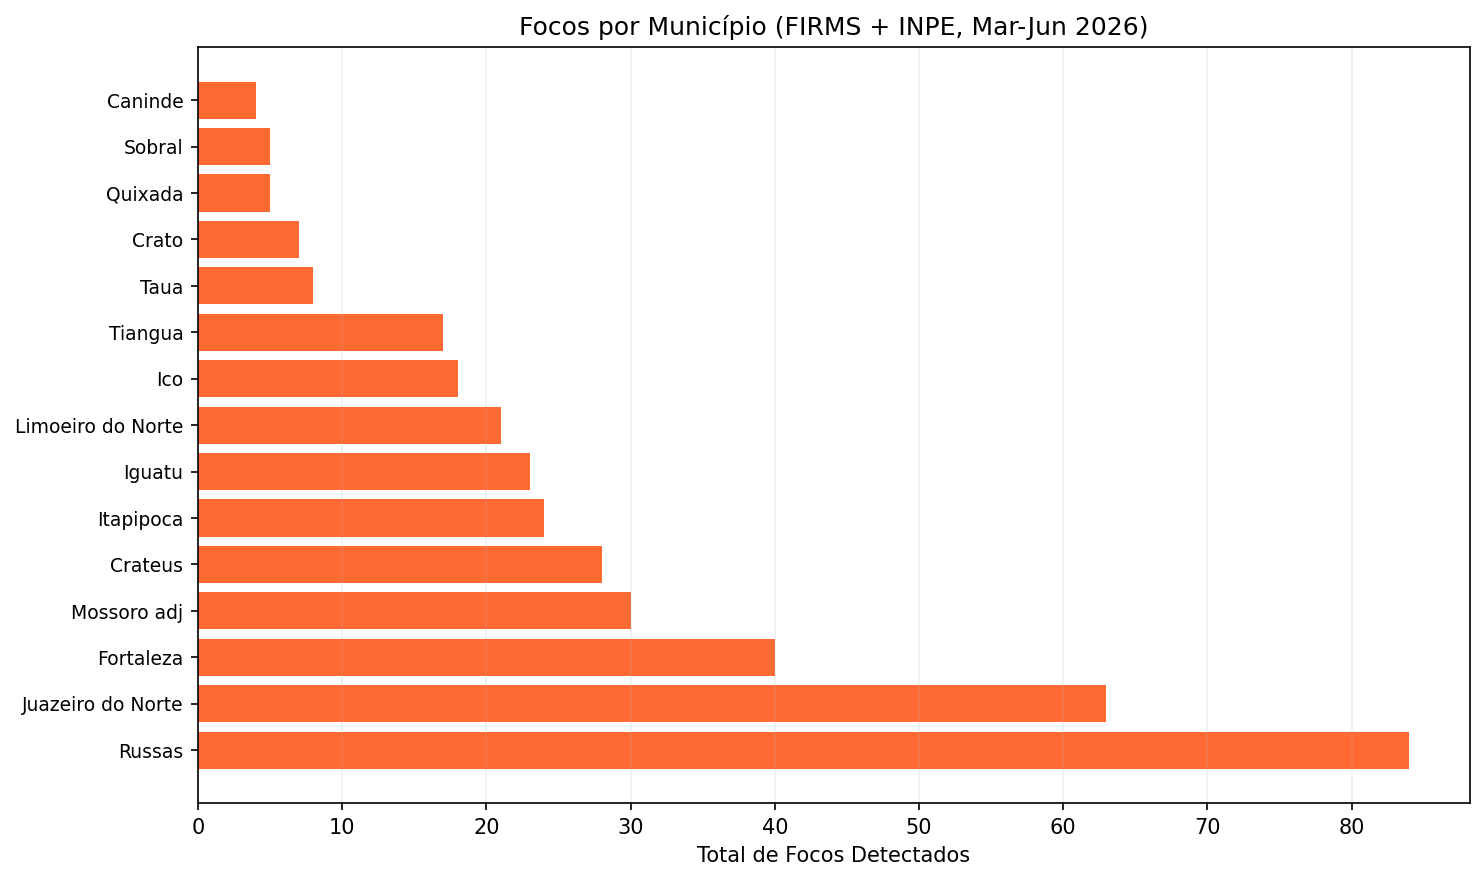
\includegraphics[width=0.75\linewidth]{figures/experimentos/05_focos_por_municipio.png}
\caption{Hotspots per monitored municipality (Exp-B real-data subset, Mar--Jun/2026).}
\label{fig:municipios-appendix}
\end{figure}

Table~\ref{tab:exp-v1} records the initial synthetic benchmark where KL-regularized Koopman-VAE underperformed shallow baselines. Table~\ref{tab:exp-v4} shows that feature expansion degraded MLP performance under data scarcity (62--67 training samples).

\begin{resulttable}{Exp-B v1: synthetic regression (200 steps, 20 nodes).}{tab:exp-v1}
\begin{tabular}{@{}lcccc@{}}
\toprule
\textbf{Model} & \textbf{RMSE}$\downarrow$ & \textbf{R\textsuperscript{2}}$\uparrow$ & \textbf{F1} & \textbf{Recall} \\
\midrule
MLP & \textbf{0.083} & \textbf{0.932} & 0.957 & 0.941 \\
XGBoost & 0.085 & 0.929 & \textbf{0.958} & 0.945 \\
Koopman-VAE (ours) & 0.260 & 0.343 & 0.828 & 0.989 \\
NeKo-PIGNN (ours) & 0.272 & 0.276 & 0.830 & 0.989 \\
\bottomrule
\end{tabular}
\end{resulttable}

\begin{resulttable}{Exp-B v4: real-data regression with feature-engineering variants.}{tab:exp-v4}
\begin{tabular}{@{}lcccc@{}}
\toprule
\textbf{Model} & \textbf{RMSE}$\downarrow$ & \textbf{R\textsuperscript{2}}$\uparrow$ & \textbf{F1} & \textbf{Precision} \\
\midrule
MLP plain & \textbf{0.143} & \textbf{0.782} & 0.936 & 0.911 \\
XGBoost + FeatEng & 0.149 & 0.767 & 0.935 & 0.902 \\
Ensemble (NeKo+XGB) & 0.149 & 0.766 & 0.930 & 0.896 \\
NeKo-PIGNN v3 & 0.173 & 0.686 & 0.906 & 0.907 \\
MLP + FeatEng + LB7 & 0.276 & 0.197 & 0.830 & 0.936 \\
\bottomrule
\end{tabular}
\end{resulttable}

Tables~\ref{tab:exp-v5}--\ref{tab:exp-v7} trace the rare-event detection iteration: v5 introduces Average Precision optimization; v6 adds focal loss and conservative XGBoost; v7 incorporates the persistence prior that raised precision to 47.5\% with only 21 false positives.

\begin{resulttable}{Exp-B v5: rare-event detection --- Average Precision and threshold metrics.}{tab:exp-v5}
\begin{tabular}{@{}lccccc@{}}
\toprule
\textbf{Model} & \textbf{AP}$\uparrow$ & \textbf{F1@best} & \textbf{Prec.} & \textbf{Recall} & \textbf{FP@0.3} \\
\midrule
MLP & 0.291 & 0.348 & 0.212 & 0.978 & 270 \\
NeKo-PIGNN v5 & \textbf{0.353} & 0.323 & \textbf{0.385} & 0.278 & \textbf{39} \\
XGBoost & 0.304 & 0.295 & 0.349 & 0.256 & 43 \\
Ensemble (NeKo+MLP) & \textbf{0.325} & \textbf{0.345} & 0.455 & 0.278 & --- \\
\bottomrule
\end{tabular}
\end{resulttable}

\begin{resulttable}{Exp-B v6: precision--recall operating modes.}{tab:exp-v6}
\begin{tabular}{@{}lccccc@{}}
\toprule
\textbf{Model} & \textbf{AP} & \textbf{F1@best} & \textbf{Prec.} & \textbf{Recall} & \textbf{FP@0.3} \\
\midrule
XGBoost (300 trees) & \textbf{0.322} & \textbf{0.427} & \textbf{0.335} & 0.589 & \textbf{28} \\
Ensemble (NeKo+XGB+MLP) & 0.315 & 0.353 & 0.217 & \textbf{0.956} & 67 \\
NeKo-PIGNN (5-seed avg.) & 0.280 & 0.324 & 0.233 & 0.533 & 81 \\
MLP (5-seed) & 0.276 & 0.350 & 0.213 & 0.989 & 282 \\
\bottomrule
\end{tabular}
\end{resulttable}

\begin{resulttable}{Exp-B v7: persistence prior combined with ML ensemble.}{tab:exp-v7}
\begin{tabular}{@{}lcccc@{}}
\toprule
\textbf{Model} & \textbf{Precision} & \textbf{Recall} & \textbf{F1} & \textbf{FP} \\
\midrule
Persistence only & 45.1\% & 48.7\% & 0.469 & 45 \\
Ensemble $\times$ Persistence & \textbf{47.5\%} & 21.1\% & 0.292 & \textbf{21} \\
NeKo $\times$ Persistence & 40.7\% & 24.4\% & 0.306 & 32 \\
XGBoost raw & 33.5\% & 58.9\% & 0.427 & 105 \\
\bottomrule
\end{tabular}
\end{resulttable}

Table~\ref{tab:three-class-full} reports per-class precision/recall/F1 from argmax classification; operational YES alerts use $P(\text{YES})\geq 0.30$ instead (Section~\ref{sec:three-level}). Table~\ref{tab:ablation-neko} confirms synergistic Koopman--PI-GNN coupling (full F1 = 0.914 vs.\ Koopman-only 0.820).

\begin{resulttable}{Full three-class classification report (Exp-B v9, XGBoost, 420 samples).}{tab:three-class-full}
\begin{tabular}{@{}lcccc@{}}
\toprule
\textbf{Class} & \textbf{Precision} & \textbf{Recall} & \textbf{F1} & \textbf{Support} \\
\midrule
NO & 0.693 & 0.973 & 0.810 & 186 \\
UNCERTAIN & 0.669 & 0.674 & 0.671 & 144 \\
YES & 0.500 & 0.078 & 0.135 & 90 \\
\midrule
Macro avg & 0.621 & 0.575 & 0.539 & 420 \\
Weighted avg & 0.644 & 0.679 & 0.618 & 420 \\
\bottomrule
\multicolumn{5}{@{}l@{}}{\textit{Note:} Operational YES alerts use $P(\text{YES})\geq 0.3$ (82.1\% precision), not argmax class.} \\
\end{tabular}
\end{resulttable}

\begin{resulttable}{NeKo-PIGNN component ablation on synthetic Rothermel propagation data.}{tab:ablation-neko}
\begin{tabular}{@{}lcccc@{}}
\toprule
\textbf{Model} & \textbf{F1} & \textbf{IoU} & \textbf{RMSE} & \textbf{R\textsuperscript{2}} \\
\midrule
NeKo-PIGNN (full) & 0.9140 & 0.8418 & 0.1083 & 0.8102 \\
Koopman-only & 0.8200 & 0.6949 & 0.1531 & 0.6215 \\
PI-GNN-only & 0.7900 & 0.6529 & 0.1682 & 0.5394 \\
Pure GNN & 0.3678 & 0.2255 & 0.2851 & $-0.32$ \\
CNN U-Net & 0.4599 & 0.2990 & 0.2514 & $-0.03$ \\
\bottomrule
\end{tabular}
\end{resulttable}


%% ===================================================================
%% References (Elsevier BibTeX — Ecological Informatics)
%% ===================================================================
\bibliographystyle{elsarticle-num}
\bibliography{submission/refs-ems}

\end{document}